\documentclass{amsart}
%\documentclass[a4paper,10pt]{scrartcl}

\usepackage[utf8x]{inputenc}
\usepackage[british]{babel}
\usepackage[a4paper, inner=2.5cm, outer=2.5cm, top=1cm,
bottom=1.5cm, bindingoffset=1cm]{geometry}
\usepackage{amsmath}
\usepackage{amssymb, latexsym}
\usepackage{longtable}
\usepackage[table]{xcolor}
\usepackage{textcomp} 
\usepackage{stmaryrd}
\usepackage{graphicx}
\usepackage{enumitem}
\usepackage{yfonts}
\usepackage{algpseudocode}
\usepackage{algorithm}
\usepackage{tikz}
\usepackage{hyperref}
\usepackage{MnSymbol}

% \setlist[enumerate]{label*=\arabic*.}
% \newtheorem{theorem}{Theorem}[section]
% \newtheorem{example}{Example}[section]
% \newtheorem{definition}{Definition}[section]
% \newtheorem{proposition}{Proposition}[section]
% \newtheorem{notation}{Notation}[section]

\renewcommand{\algorithmicrequire}{\textbf{Input:}}
\renewcommand{\algorithmicensure}{\textbf{Output:}}


\newcommand\armstrong[1][]{%
\tikzset{
    shield width/.store in=\shieldwidth,
    shield width=0.8ex,
    shield height/.store in=\shieldheight,
    shield height=1ex
}%
\tikz [baseline,#1] \draw (0,\shieldheight) -- (0,\shieldwidth/2) arc [radius=\shieldwidth/2, start angle=-180, end angle=0] -- (\shieldwidth,\shieldheight) -- cycle;%
}

\newcommand{\defined}{\mathrel{\mathop:}=}

\newcommand\tableEntailmentSpacing{2.5cm}
\newcommand\tableExamplarSpacing{3.5cm}
\newcommand\tableCommentSpacing{4cm}
\newcommand\tableEquationIndent{4pt}

% \allowdisplaybreaks

\title{}
\author{}
\date{}

\pdfinfo{%
  /Title    (Application of Armstrong ABoxes for ALC TBoxes)
  /Author   (Henriette Harmse)
  /Creator  ()
  /Producer ()
  /Subject  (DL)
  /Keywords (Armstrong ABoxes)
}

\begin{document}
  \maketitle
  
  \section{Armstrong ABoxes}
  
  \subsection{A Quick Review of the Armstrong ABox Algorithm}
    The Armstrong ABox algorithm is based on ontology completion algorithm of Baader, et al, which is based on partial contexts, which in turn is based on the attribute exploration algorithm of FCA. Recall that an FCA formal context can be visualised as a crosstable, where the rows represent the objects, and the columns represent the attributes. A cross in column $m$ of row $g$ means that object $g$ has attribute $m$, absence of a cross means that object $g$ does not have attribute $m$.   
    The purpose of attribute exploration is to complete an FCA context by (1) creating an implication base of implications that hold in the context and (2) adding counter examples for implications that do not hold in the context. 
%     Counter examples in FCA are FCA objects and objects in FCA can have attributes. 
    For an FCA context consisting of attributes $M = \{m_1, \ldots, m_n\}$ implications are considered one-by-one, starting from the implication $\top \rightarrow \{m_1, \ldots, m_n\}$ and iterating through the unrefuted implications in the lectic order till it reaches $\{m_1, \ldots, m_n\} \rightarrow \top$. 
    
    
    For Armstrong ABoxes the underlying context is based on a partial context where the context consists of the Armstrong ABox $\mathcal{A}_{\armstrong}$, the attributes of the context is given by $M = \{m_1, \ldots, m_n\}$ where the elements of $M$ are concepts, and the objects of the context are given by the individuals and their assertions in $\mathcal{A}_{\armstrong}$. Similar to the attribute exploration algorithm of FCA, the Armstrong ABox algorithm constructs an implication base of the implications (equivalently the subsumptions) that hold in the context. The Armstrong ABox algorithm constructs the Armstrong ABox $\mathcal{A}_{\armstrong}$ by checking whether the subsumption statements constructed based on $M$ are entailed by the associated TBox $\mathcal{T}$. If the subsumption statement  $\bigsqcap C_i \sqsubseteq \bigsqcap D_ j$ follows from $\mathcal{T}$, the implication $C_i \rightarrow D_j$ is added to the implication base, otherwise a violating exemplar is added to $\mathcal{A}_{\armstrong}$. The algorithm traverses the subsumption statements in the lectic order from $m_1 \sqcup \ldots \sqcup m_n \sqsubseteq m_1 \sqcap \ldots \sqcap m_n$ to $m_1 \sqcap \ldots \sqcap m_n \sqsubseteq m_1 \sqcup \ldots \sqcup m_n$.   
  
  \subsection{Limitations of Armstrong ABoxes for ALC TBoxes} \label{subsec_ArmstrongABoxLimitations}
  Armstrong ABoxes have some limitations that we discuss here.
  \subsection{Only support ALC TBoxes}
  Currently Armstrong ABoxes can only be generated for $\mathcal{ALC}$ TBoxes. However, constructors often used in public ontologies (see Table~\ref{tab_PublicOntologies}) include role hierarchies, inverse roles, functional role restrictions, transitive roles and data types. Of these the most useful seem to be role hierarchies, inverse roles and data types. Inverse roles can be particularly helpful in identifying missing range restrictions. Functional role restrictions are often used in UML class diagrams and for that reason they are also of importance.
  
  
       \rowcolors{1}{white}{lightgray}
   \begin{table}
   \footnotesize
 %     \scriptsize
     \begin{center} 
       \caption{Armstrong ABox for $\mathcal{T}_0$ and $M=\{\mathsf{Person}, \mathsf{Person} \sqcup \mathsf{Course}\}$}
       \label{tab_PublicOntologies}
       \smallskip
       \begin{tabular}
       {|>{\footnotesize}p{8cm}|>{\footnotesize}p{3cm}|}
       \hline
       \multicolumn{1}{|>{\footnotesize}c|}{\textbf{Ontology}}&{\textbf{DL Used}}\\
       \hline       
        Dublin Core (DC)~\cite{DublinCore} & $\mathcal{ALH}(\mathcal{D})$\\
        Friend Of A Friend (FOAF)~\cite{FOAF} & $\mathcal{ALCHIF}(\mathcal{D})$\\
        Gene Ontology (GO)~\cite{GeneOntology} & $\mathcal{SRI}$\\
        GoodRelations~\cite{GoodRelations_v1} & $\mathcal{SHI}(\mathcal{D})$\\
        MarineTLO~\cite{MarineTLOv5} & $\mathcal{ALCHIF}(\mathcal{D})$ \\
        SNOMED & OWL 2 EL / $\mathcal{EL}^{++}$ \\
        Socially Interconnected Online Communities (SOIC)~\cite{SIOC} &  $\mathcal{SHI}(\mathcal{D})$ \\
       \hline      
       \end{tabular}
     \end{center}
     \normalsize
   \end{table} 
   
   \subsection{The Revised M-permissible Restriction} \label{subsec_MPermissibleRestriction} 
   For a role $r$ the potential domain restrictions can be explored by analysing how the concept $\exists r.\top$ relates to candidate domains. For example, if it is suspected that $D$ is a domain of $r$, an Armstrong ABox can be generated for the related TBox and $M := \{\exists r.\top, D\}$. Due to the $M$-permissible restriction, Armstrong ABoxes cannot be used to analyse range restrictions in a similar way.

   In $\mathcal{ALC}$ one can state that role $r$ has range $D$ by adding the axiom $\top \sqsubseteq \forall r. D$ to the TBox. Since $M$-permissible excludes $\top$, or any concept that is equivalent to $\top$, from being an element of $M$, there is no way to analyse range restrictions using Armstrong ABoxes.
   
   One possible way to enable Armstrong ABoxes to analyse range restrictions is to extend Armstrong ABoxes to $\mathcal{ALCI}$. This will allow range restrictions to be expressed as $\exists r^-.\top \sqsubseteq D$, which we then can analyse using $M := \{\exists r^-.\top, D\}$. 
  
  \subsection{The Disadvantage of Optimal Counterexamples - The Case for Keeping M Small} 
  When the Armstrong ABox algorithm encounters a non-entailment, it automatically generates a violating exemplar that is an optimal counterexample of the entailment that does not follow from the TBox. For example, if for a TBox $\mathcal{T}$ we have the non-entailment $\mathcal{T} \nvDash \bigsqcap C_i \sqsubseteq \bigsqcap D_j$, a violating exemplar of the form $\{(\bigsqcap C_i)(x), \neg(\bigsqcap D_j)(x)\}$ is generated. We say the violating exemplar represented by $x$ is an optimal counterexample because it refutes $\bigsqcap C_i \sqsubseteq \bigsqcap D_j$ for all $D_j$. That is we know that $\mathcal{T} \nvDash \bigsqcap C_i \sqsubseteq D_1$, or $\mathcal{T} \nvDash \bigsqcap C_i \sqsubseteq D_2$, $\ldots$, or $\mathcal{T} \nvDash \bigsqcap C_i \sqsubseteq D_m$ for $0 \leq j \leq m$. An example of a non-optimal counterexample is $\{(\bigsqcap C_i)(x), \neg (D_1 \sqcap D_2)(x)\}$, which refutes $\mathcal{T} \vDash \bigsqcap C_i \sqsubseteq  D_1 \sqcap D_2$ which implies that $\mathcal{T} \nvDash \bigsqcap C_i \sqsubseteq D_1$, or $\mathcal{T} \nvDash \bigsqcap C_i \sqsubseteq D_2$. From an Armstrong ABox (and ontology completion) algorithm perspective it still needs to refute $\bigsqcap C_i \sqsubseteq D_3 \sqcap \ldots \sqcap D_m$.
  
  The advantage of a violating exemplar that is an optimal counterexample is that the domain expert only needs to review one violating exemplar which consists of a maximum of two assertions for a given non-entailment. The disadvantage is that it could hide a smaller non-entailment, that if the domain expert was presented with it, could have resulted in the domain expert realizing that it must be an axiom of the application domain.
  
  Naturally we could have defined a violating exemplar for $\mathcal{T} \nvDash \bigsqcap C_i \sqsubseteq \bigsqcap D_j$ as 
  \[(\bigsqcap C_i)(x_1), (\neg D_1)(x_1), \ldots,(\bigsqcap C_i)(x_m), (\neg D_m)(x_m),\]
  assuming $1 \leq j \leq m$. The disadvantage of this formulation is that the domain expert will have a factor $m$ increase in assertions to review. The advantage is that reviewing assertions of the form $\{(\bigsqcap C_i)(x_j), (\neg D_j)(x_j)\}$ may be more intuitive to a domain expert (due to the shorter length of the negative assertion) than reviewing assertions of the form $\{(\bigsqcap C_i)(x), \neg(\bigsqcap D_j)(x)\}$.
  
  We can deal with the current formulation of violating exemplars (as an optimal counterexample) by choosing $M$ to be small. This has the following advantages:
  \begin{enumerate}
   \item A small $M$ reduces the number of potential smaller non-entailments hidden in a larger non-entailment.
   \item A small $M$ reduces the cognitive load for both the ontology engineer and the domain expert by limiting the number of concepts that a person needs to keep in mind at a given time.
  \end{enumerate}

  \subsection{M as a Singleton Set is not Helpful} 
  It is possible to generate an Armstrong ABox for a TBox and $M$ where $M$ is a singleton set. However, generating such an Armstrong ABox is not useful because for $M = {m_1}$ it will iterate through the subsumptions $m_1 \sqsubseteq m_1$ to $m_1 \sqsubseteq m_1$, which represents a single subsumption statement that is a tautology.
   
 \section{Analysing an $\mathcal{ALC}$ TBox using Armstrong ABoxes}
 \subsection{An Approach for Analysing $\mathcal{ALC}$ TBoxes using Armstrong ABoxes}
  One of the challenges in analysing an $\mathcal{ALC}$ TBox using Armstrong ABoxes is how does one choose which concept descriptions must form part of $M$? It will be beneficial if we can define an approach for choosing $M$. However, the number of sets of $M$ of interesting concepts that can be generated for a given signature of a TBox $\mathcal{T}$ is infinite. Hence, such an approach is elusive. The best we can do is provide some potential guidelines, but these guidelines are non-prescriptive.
  
  
  From a cognitive perspective evaluating the appropriateness of entailments and non-entailments for a particular application domain can be a difficult task. To ease the cognitive load Armstrong ABoxes provide satisfying- and violating exemplars to illustrate entailments and non-entailments. However, even then it can still be difficult to evaluate each exemplar.  For this reason it is a good idea to keep the number of concepts considered in $M$ small. 
  
  When deciding which concepts to include in $M$, identify one named concept that is of interest or in need of detailed investigation. For convenience we will refer to this concept as $C$. To analyse $C$ using Armstrong ABoxes, proceed in the following way:
    \begin{enumerate}
    \item Add $C$, as well as concepts that are siblings of $C$, to $M$. Siblings are the concepts that have the same direct subsumers as $C$. Revise the TBox and regenerate the Armstrong ABox until the Armstrong ABox is appropriate for the application domain with respect to the siblings of $C$.
    \item To analyse how $C$ relates to its direct subsumees,  we assume the direct subsumees of $C$ are $C_1, \ldots, C_k$.
    \begin{enumerate}
     \item \label{enum_cover} In order to determine whether the individuals in $C_1, \ldots, C_k$ represent all individuals in $C$, we generate an Armstrong ABox for the related TBox and $M = \{C, C_1 \sqcup \ldots \sqcup C_k\}$. 
     \item \label{enum_intersect} To determine whether $C_1, \ldots, C_k$ share individuals, we generate a Armstrong ABoxes for the related TBox and $M = \{C, C_1 \sqcap \ldots \sqcap C_k\}$.
     \item \label{enum_subsumee_relation}We analyse how the direct subsumees of $C$ relates to each other by generating an Armstrong ABox for the related TBox and $M = \{C_1, \ldots, C_k\}$. Note that we do not include $C$ in $M$ because we already know $C$ subsumes $\{C_1, \ldots, C_k\}$. 
     \item We analyse the GCIs in which $C$ appears by considering each GCI separately with $M$ consisting only of the subsumee and subsumer of the GCI. 
     When the subsumee and/or subsumer consist of multiple conjuncts, it may be worth  adding each conjunct as separate elements to $M$.
     \item Continue in this way down the subsumption hierarchy until $C$ is refined appropriately for the needs of the application domain.
    \end{enumerate}    
    \end{enumerate}
    
    Note that we could possibly handle steps \ref{enum_intersect} and \ref{enum_subsumee_relation} as a single step. That is, we could generate an Armstrong ABox for the TBox and $M = \{C,  C_1, \ldots, C_k, C_1 \sqcap \ldots \sqcap C_k\}$. However, this will increase the length of the assertions that the ontology engineer and domain expert have to evaluate, which could become (from a cognitive perspective) untenable.
  
  
  \subsection{Example Ontology}
  In the following we will illustrate how Armstrong ABoxes for $\mathcal{ALC}$ TBoxes can be used to analyse and refine an $\mathcal{ALC}$ TBox. 
  
%  We assume we want to create an ontology that reflects the assumptions of our application domain correctly. For our application domain we assume a university setting, where we have students and teachers. Students attend courses and teacher teach courses. Teachers may decide to  further their studies and hence they may be students as well. Courses are divided into undergraduate courses and postgraduate courses. Undergraduate courses cannot be postgrad
  
  We assume we have the TBox as defined by $\mathcal{T}_0$. 
   \begin{align*}
  \mathcal{T}_0 = \{\mathsf{Course} &\sqsubseteq \neg \mathsf{Person},\\
  \mathsf{Teacher} &\equiv \mathsf{Person} \sqcap \exists\mathsf{teaches}.\mathsf{Course}, \\
  \exists\mathsf{teaches}.\top &\sqsubseteq \mathsf{Person},\\
  \mathsf{Student} &\equiv \mathsf{Person} \sqcap \exists\mathsf{attends}.\mathsf{Course}, \\
  \exists\mathsf{attends}.\top &\sqsubseteq \mathsf{Person},\\ 
  \mathsf{UGCourse} &\sqsubseteq \mathsf{Course},\\
  \mathsf{PGCourse} &\sqsubseteq \mathsf{Course},\\
   \mathsf{UGStudent} &\sqsubseteq \neg\mathsf{PGStudent},\\
  \mathsf{UGStudent} &\equiv\mathsf{Student} \sqcap  \forall\mathsf{attends}.\mathsf{UGCourse},\\
  \mathsf{PGStudent} &\equiv \mathsf{Student} \sqcap \forall\mathsf{attends}.\mathsf{PGCourse}\}
  \end{align*}  
  
This ontology attempts to model a university application domain. It has the concepts $\mathsf{Person}$ and $\mathsf{Course}$ that are disjoint. It defines the $\mathsf{Teacher}$ concept as a $\mathsf{Person}$ that $\mathsf{teaches}$ a $\mathsf{Course}$. A $\mathsf{Student}$ is modelled as a $\mathsf{Person}$ who $\mathsf{attends}$ a $\mathsf{Course}$. Undergraduate courses are represented by the concept $\mathsf{UGCourse}$ and postgraduate courses are represented by the concept $\mathsf{PGCourse}$. Undergraduate students ($\mathsf{UGStudent}$) are students that attend only undergraduate courses and postgraduate students ($\mathsf{PGStudent}$) are students that only attend postgraduate courses. Undergraduate students are not postgraduate students and vice versa.

  \subsection{Analysing the $\mathsf{Person}$ Concept}
  
       \rowcolors{1}{white}{lightgray}
   \begin{table}
   \footnotesize
 %     \scriptsize
     \begin{center} 
       \caption{Armstrong ABox for $\mathcal{T}_0$ and $M=\{\mathsf{Person}, \mathsf{Course}\}$}
       \label{tab_ArmstrongABox_Person_Course}
       \smallskip
       \begin{tabular}
       {|>{\footnotesize}p{\tableEntailmentSpacing}|>{\footnotesize}p{\tableExamplarSpacing}|>{\footnotesize}p{\tableExamplarSpacing}|>{\footnotesize}p{\tableCommentSpacing}|}
       \hline
        \multicolumn{1}{|>{\footnotesize}c|}{\textbf{Non-entailment}}&\multicolumn{2}{>{\footnotesize}c|}{\textbf{Violating exemplar}}&\multicolumn{1}{>{\footnotesize}c|}{\textbf{Comment}}\\
        \hline
        \begin{minipage}{\tableEntailmentSpacing}
%             \vspace{2pt}
            $\begin{aligned}
              &\mathsf{Person} \sqcup \mathsf{Course}\\ 
  	      &\sqsubseteq\\
  	      &\mathsf{Person} \sqcap \mathsf{Course}
           \end{aligned}$
  	\end{minipage}
        &
        \begin{minipage}{\tableExamplarSpacing}
  	    $\begin{aligned}
  	    &(\mathsf{Person} \sqcup \mathsf{Course})(x_1)
  	    \end{aligned}$
  	\end{minipage}
  	&
  	\begin{minipage}{\tableExamplarSpacing}
  	    \vspace{2pt}
  	   $\begin{aligned}
             &\neg(\mathsf{Person} \sqcap \mathsf{Course})(x_1)
  	    \end{aligned}$ 
  	\end{minipage}
        &
        \begin{minipage}{\tableCommentSpacing}
            \vspace{2pt}
            It is possible in the application domain that there are individuals that are persons or courses, but that are either not a person or not course. This is correct for our application domain since persons are not courses and courses are not persons.
            \vspace{2pt}
        \end{minipage}     
        
  	 \\  	 
  	 
        \begin{minipage}{\tableEntailmentSpacing}
%             \vspace{2pt}
            $\begin{aligned}
              &\mathsf{Course}\sqsubseteq\mathsf{Person}
           \end{aligned}$
  	\end{minipage}
        &
        \begin{minipage}{\tableExamplarSpacing}
  	    $\begin{aligned}
  	    &(\mathsf{Course})(x_2)
  	    \end{aligned}$
  	\end{minipage}
  	&
  	\begin{minipage}{\tableExamplarSpacing}
  	    \vspace{2pt}
  	   $\begin{aligned}
             &\neg(\mathsf{Person})(x_2)
  	    \end{aligned}$ 
  	\end{minipage}
        &
        \begin{minipage}{\tableCommentSpacing}
            \vspace{2pt}
            It is possible in the application domain that there are individuals that are courses, but that are not persons, which agrees with the assumptions for our application domain.
            \vspace{2pt}
        \end{minipage}  	 
        \\
        \begin{minipage}{\tableEntailmentSpacing}
%             \vspace{2pt}
            $\begin{aligned}
              &\mathsf{Person}\sqsubseteq\mathsf{Course}
           \end{aligned}$
  	\end{minipage}
        &
        \begin{minipage}{\tableExamplarSpacing}
  	    $\begin{aligned}
  	    &(\mathsf{Person})(x_3)
  	    \end{aligned}$
  	\end{minipage}
  	&
  	\begin{minipage}{\tableExamplarSpacing}
  	    \vspace{2pt}
  	   $\begin{aligned}
             &\neg(\mathsf{Course})(x_3)
  	    \end{aligned}$ 
  	\end{minipage}
        &
        \begin{minipage}{\tableCommentSpacing}
            \vspace{2pt}
            It is possible in the application domain that there are individuals that are persons, but that are not courses. This is correct for our application domain.     
            \vspace{2pt}
        \end{minipage}  	 
        \\        
        \hline      
       \end{tabular}
     \end{center}
     \normalsize
   \end{table}
   
  We start by identifying a concept of interest, which we assume is the $\mathsf{Person}$ concept. We start our analysis of the $\mathsf{Person}$ concept by considering its relation to its siblings.
  The only sibling of $\mathsf{Person}$ is $\mathsf{Course}$, we therefore include $\mathsf{Course}$ in $M$.  
  Hence, we start our analysis of $\mathsf{Person}$ by generating an Armstrong ABox for $\mathcal{T}_0$ and $M := \{\mathsf{Person}, \mathsf{Course}\}$, which is given in Table~\ref{tab_ArmstrongABox_Person_Course}. This Armstrong ABox consists only of violating exemplars. Moreover, the violating exemplars agree with our understanding of the application domain and hence we leave the TBox unchanged.
   
We now consider how the $\mathsf{Person}$ concept relates to its direct subsumees, $\mathsf{Student} $ and $\mathsf{Teacher}$. To determine whether the individuals in the union of $\mathsf{Student}$ and $\mathsf{Teacher}$ represent all the individuals of the $\mathsf{Person}$ concept, we generate an Armstrong ABox for $\mathcal{T}_0$ and  $M = \{\mathsf{Person}, \mathsf{Student} \sqcup \mathsf{Teacher}\}$, which is represented in Table~\ref{tab_ArmstrongABox_Person_StudentORTeacher}. This Armstrong ABox consists of a violating exemplar and a satisfying examplar, where the application domain agrees with the satisfying exemplar, but not with the violating exemplar. The violating exemplar indicates that it is possible in the application domain that there is an individual that is a person or a student or a teacher, that is not a person, or that is not a student and not a teacher. If we assume for our application domain we only deal with persons who are students and/or teachers, this statement is incorrect. We can revise our TBox by adding the axiom 
\[\mathsf{Person} \sqcup (\mathsf{Student} \sqcup \mathsf{Teacher}) \sqsubseteq \mathsf{Person} \sqcap (\mathsf{Student} \sqcup \mathsf{Teacher}).\]
However, in this case it may be more intuitive to add the axiom
     \[\mathsf{Person} \equiv \mathsf{Student} \sqcup \mathsf{Teacher}\]
to the TBox. In many instances, where a violating exemplar does not agree with the assumptions of the application domain, it may be possible to add an axiom corresponding to the non-entailment to the TBox. Though, it is not possible in all cases, since adding an axiom corresponding to the non-entailment to the TBox may cause the TBox to become inconsistent. Hence, a less restrictive axiom derived from the non-entailment may need to be added. Moreover, the ontology engineer (in collaboration with the domain expert) may decide to add a more restrictive axiom (or axioms), assuming it does not result in the TBox becoming inconsistent. Another viable action is to revise an existing axiom (or axioms). The point is that when the assumptions of the application domain disagree with a violating exemplar, it indicates to an ontology engineer and domain expert where efforts for fine tuning the ontology must be spent. It does not indicate the exact action required to resolve the disagreement.

For our example we will opt to add the axiom
 \[\mathsf{Person} \equiv \mathsf{Student} \sqcup \mathsf{Teacher}\]
to the TBox, with the revised TBox defined  as $\mathcal{T}_1$.
The result of the Armstrong ABox generated for $\mathcal{T}_1$ and $M=\{\mathsf{Person}, \mathsf{Student} \sqcup \mathsf{Teacher}\}$ is given in Table~\ref{tab_ArmstrongABox_Person_StudentORTeacher_Revised}. The fact that the violating exemplar of Table~\ref{tab_ArmstrongABox_Person_StudentORTeacher} no longer appears in Table~\ref{tab_ArmstrongABox_Person_StudentORTeacher_Revised}, indicates that adding the axiom has resolved the disagreement. Moreover, the satisfying exemplars confirm that (1) persons are students or teachers, (2) students are persons and (3) teachers are persons.

     
     \rowcolors{1}{white}{lightgray}
   \begin{table}
   \footnotesize
 %     \scriptsize
     \begin{center} 
       \caption{Armstrong ABox for $\mathcal{T}_0$ and $M=\{\mathsf{Person}, \mathsf{Student} \sqcup \mathsf{Teacher}\}$}
       \label{tab_ArmstrongABox_Person_StudentORTeacher}
       \smallskip
       \begin{tabular}
       {|>{\footnotesize}p{\tableEntailmentSpacing}|>{\footnotesize}p{\tableExamplarSpacing}|>{\footnotesize}p{\tableExamplarSpacing}|>{\footnotesize}p{\tableCommentSpacing}|}
       \hline
        \multicolumn{1}{|>{\footnotesize}c|}{\textbf{Entailment}}&\multicolumn{2}{>{\footnotesize}c|}{\textbf{Satisfying exemplar}}&\multicolumn{1}{>{\footnotesize}c|}{\textbf{Comment}}\\
        \hline
        \begin{minipage}{\tableEntailmentSpacing}
        \vspace{2pt}
            $\begin{aligned}
              &\mathsf{Student}  \sqcup \mathsf{Teacher} \\
  	      &\sqsubseteq\\
  	      &\mathsf{Person}
           \end{aligned}$
  	\end{minipage}
        &
        \begin{minipage}{\tableExamplarSpacing}
  	    $\begin{aligned}
               &(\mathsf{Student}  \sqcup \mathsf{Teacher})(x_2)
  	    \end{aligned}$
  	\end{minipage}
  	&
  	\begin{minipage}{\tableExamplarSpacing}
  	    \vspace{2pt}
  	   $\begin{aligned}
             &\mathsf{Person}(x_2)
  	    \end{aligned}$ 
  	\end{minipage}
        &
        \begin{minipage}{\tableCommentSpacing}
            \vspace{2pt}
            Individuals that are students or teachers, are persons, which is true.
            \vspace{2pt}
        \end{minipage}     
        \\
        \hline
        \multicolumn{1}{|>{\footnotesize}c|}{\textbf{Non-entailment}}&\multicolumn{2}{>{\footnotesize}c|}{\textbf{Violating exemplar}}&\multicolumn{1}{>{\footnotesize}c|}{\textbf{Comment}}\\
        \hline
        \begin{minipage}{\tableEntailmentSpacing}
%             \vspace{2pt}
            $\begin{aligned}
              &\mathsf{Person} \hspace{2pt} \sqcup \\
              &\hspace{\tableEquationIndent}(\mathsf{Student} \sqcup \mathsf{Teacher})\\ 
  	      &\sqsubseteq\\
  	      &\mathsf{Person} \hspace{2pt} \sqcap \\
  	      &\hspace{\tableEquationIndent}(\mathsf{Student} \sqcup \mathsf{Teacher})
           \end{aligned}$
  	\end{minipage}
        &
        \begin{minipage}{\tableExamplarSpacing}
  	    $\begin{aligned}
               &(\mathsf{Person} \hspace{2pt} \sqcup \\
               &\hspace{\tableEquationIndent}(\mathsf{Student} \sqcup \mathsf{Teacher}))(x_1)
  	    \end{aligned}$
  	\end{minipage}
  	&
  	\begin{minipage}{\tableExamplarSpacing}
  	    \vspace{2pt}
  	   $\begin{aligned}
             &\neg(\mathsf{Person} \hspace{2pt} \sqcap \\
             &\hspace{\tableEquationIndent}(\mathsf{Student} \sqcup \mathsf{Teacher}))(x_1)
  	    \end{aligned}$ 
  	\end{minipage}
        &
        \begin{minipage}{\tableCommentSpacing}
            \vspace{2pt}
            It is possible in the application domain that there is an individual that is a person or a student or a teacher, that is not a person, or that is not a student and not a teacher. If we assume our application domain only deals with persons who are students and/or teachers, this statement is false.
            \vspace{2pt}
        \end{minipage}     
        \\
         \hline      
       \end{tabular}
     \end{center}
     \normalsize
   \end{table}
  

   \begin{align*}
  \mathcal{T}_1 = \{\mathsf{Course} &\sqsubseteq \neg \mathsf{Person},\\
  \mathsf{Person} &\equiv \mathsf{Student} \sqcup \mathsf{Teacher}, \\ 
  \mathsf{Teacher} &\equiv \mathsf{Person} \sqcap \exists\mathsf{teaches}.\mathsf{Course}, \\
  \exists\mathsf{teaches}.\top &\sqsubseteq \mathsf{Person},\\
  \mathsf{Student} &\equiv \mathsf{Person} \sqcap \exists\mathsf{attends}.\mathsf{Course}, \\
  \exists\mathsf{attends}.\top &\sqsubseteq \mathsf{Person},\\ 
  \mathsf{UGCourse} &\sqsubseteq \mathsf{Course},\\
  \mathsf{PGCourse} &\sqsubseteq \mathsf{Course},\\
   \mathsf{UGStudent} &\sqsubseteq \neg\mathsf{PGStudent},\\
  \mathsf{UGStudent} &\equiv\mathsf{Student} \sqcap  \forall\mathsf{attends}.\mathsf{UGCourse},\\
  \mathsf{PGStudent} &\equiv \mathsf{Student} \sqcap \forall\mathsf{attends}.\mathsf{PGCourse}\}
  \end{align*}   
  
  
      \rowcolors{1}{white}{lightgray}
   \begin{table}
   \footnotesize
 %     \scriptsize
     \begin{center} 
       \caption{Armstrong ABox for $\mathcal{T}_1$ and $M=\{\mathsf{Person}, \mathsf{Student} \sqcup \mathsf{Teacher}\}$}
       \label{tab_ArmstrongABox_Person_StudentORTeacher_Revised}
       \smallskip
       \begin{tabular}
       {|>{\footnotesize}p{\tableEntailmentSpacing}|>{\footnotesize}p{\tableExamplarSpacing}|>{\footnotesize}p{\tableExamplarSpacing}|>{\footnotesize}p{\tableCommentSpacing}|}
       \hline
        \multicolumn{1}{|>{\footnotesize}c|}{\textbf{Entailment}}&\multicolumn{2}{>{\footnotesize}c|}{\textbf{Satisfying exemplar}}&\multicolumn{1}{>{\footnotesize}c|}{\textbf{Comment}}\\
        \hline
        \begin{minipage}{\tableEntailmentSpacing}
        \vspace{2pt}
            $\begin{aligned}
              &\mathsf{Person} \hspace{2pt} \sqcup \\
              &\hspace{\tableEquationIndent}(\mathsf{Student} \sqcup \mathsf{Teacher})\\
  	      &\sqsubseteq \\
  	      &\mathsf{Person} \hspace{2pt} \sqcap \\
  	      &\hspace{\tableEquationIndent}(\mathsf{Student} \sqcup \mathsf{Teacher})
           \end{aligned}$
  	\end{minipage}
        &
        \begin{minipage}{\tableExamplarSpacing}
  	    $\begin{aligned}
               &(\mathsf{Person} \hspace{2pt} \sqcup \\
              &\hspace{\tableEquationIndent}(\mathsf{Student} \sqcup \mathsf{Teacher}))(x_1)
  	    \end{aligned}$
  	\end{minipage}
  	&
  	\begin{minipage}{\tableExamplarSpacing}
  	    \vspace{2pt}
  	   $\begin{aligned}
             &(\mathsf{Person} \hspace{2pt} \sqcap \\
  	      &\hspace{\tableEquationIndent}(\mathsf{Student} \sqcup \mathsf{Teacher}))(x_1)
  	    \end{aligned}$ 
  	\end{minipage}
        &
        \begin{minipage}{\tableCommentSpacing}
            \vspace{2pt}
            An individual that is a person or a student or a teacher, is a person and a student, or a person and a teacher, which is true.
            \vspace{2pt}
        \end{minipage}     
        \\
        \begin{minipage}{\tableEntailmentSpacing}
        \vspace{2pt}
            $\begin{aligned}
              &\mathsf{Student} \sqcup \mathsf{Teacher}\\
  	      &\sqsubseteq\\
  	      &\mathsf{Person} 
           \end{aligned}$
  	\end{minipage}
        &
        \begin{minipage}{\tableExamplarSpacing}
  	    $\begin{aligned}
               &(\mathsf{Student} \sqcup \mathsf{Teacher})(x_2)
  	    \end{aligned}$
  	\end{minipage}
  	&
  	\begin{minipage}{\tableExamplarSpacing}
  	    \vspace{2pt}
  	   $\begin{aligned}
             &\mathsf{Person}(x_2)
  	    \end{aligned}$ 
  	\end{minipage}
        &
        \begin{minipage}{\tableCommentSpacing}
            \vspace{2pt}
            An individual that is a student or a teacher, is a person, which is true.
            \vspace{2pt}
        \end{minipage}         
        \\
        \begin{minipage}{\tableEntailmentSpacing}
        \vspace{2pt}
            $\begin{aligned}
              &\mathsf{Person}\\
  	      &\sqsubseteq\\
  	      &\mathsf{Student}  \sqcup \mathsf{Teacher}
           \end{aligned}$
  	\end{minipage}
        &
        \begin{minipage}{\tableExamplarSpacing}
  	    $\begin{aligned}
               &\mathsf{Person}(x_3)
  	    \end{aligned}$
  	\end{minipage}
  	&
  	\begin{minipage}{\tableExamplarSpacing}
  	    \vspace{2pt}
  	   $\begin{aligned}
             &(\mathsf{Student}  \sqcup \mathsf{Teacher})(x_3)
  	    \end{aligned}$ 
  	\end{minipage}
        &
        \begin{minipage}{\tableCommentSpacing}
            \vspace{2pt}
            An individual that is a person, is a student or a teacher, which is true.
            \vspace{2pt}
        \end{minipage}         
        \\
        \hline 
        
       \end{tabular}
     \end{center}
     \normalsize
   \end{table}
 
 
 We verify whether the direct subsumees of $\mathsf{Person}$ can intersect by generating an Armstrong ABox for $\mathcal{T}_1$ and $M =\{\mathsf{Person}, \mathsf{Student} \sqcap \mathsf{Teacher}\}$. The corresponding Armstrong ABox is represented by Table~\ref{tab_ArmstrongABox_Person_StudentANDTeacher}, which accurately describes the assumptions for our application domain.
 
 
        \rowcolors{1}{white}{lightgray}
   \begin{table}
   \footnotesize
 %     \scriptsize
     \begin{center} 
       \caption{Armstrong ABox for $\mathcal{T}_1$ and $M=\{\mathsf{Person}, \mathsf{Student} \sqcap \mathsf{Teacher}\}$}
       \label{tab_ArmstrongABox_Person_StudentANDTeacher}
       \smallskip
       \begin{tabular}
       {|>{\footnotesize}p{\tableEntailmentSpacing}|>{\footnotesize}p{\tableExamplarSpacing}|>{\footnotesize}p{\tableExamplarSpacing}|>{\footnotesize}p{\tableCommentSpacing}|}
       \hline
        \multicolumn{1}{|>{\footnotesize}c|}{\textbf{Entailment}}&\multicolumn{2}{>{\footnotesize}c|}{\textbf{Satisfying exemplar}}&\multicolumn{1}{>{\footnotesize}c|}{\textbf{Comment}}\\
        \hline
        \begin{minipage}{\tableEntailmentSpacing}
        \vspace{2pt}
            $\begin{aligned}
              &\mathsf{Student} \sqcap \mathsf{Teacher}\\
  	      &\sqsubseteq\\
  	      &\mathsf{Person}
           \end{aligned}$
  	\end{minipage}
        &
        \begin{minipage}{\tableExamplarSpacing}
  	    $\begin{aligned}
               &(\mathsf{Student} \sqcap \mathsf{Teacher})(x_2)
  	    \end{aligned}$
  	\end{minipage}
  	&
  	\begin{minipage}{\tableExamplarSpacing}
  	    \vspace{2pt}
  	   $\begin{aligned}
             &\mathsf{Person}(x_2)
  	    \end{aligned}$ 
  	\end{minipage}
        &
        \begin{minipage}{\tableCommentSpacing}
            \vspace{2pt}
            Individuals that are both students and teachers are persons, which is correct.
            \vspace{2pt}
        \end{minipage}     
        \\
        \hline         
        \multicolumn{1}{|>{\footnotesize}c|}{\textbf{Non-Entailment}}&\multicolumn{2}{>{\footnotesize}c|}{\textbf{Violating exemplar}}&\multicolumn{1}{>{\footnotesize}c|}{\textbf{Comment}}\\
        \hline
         \begin{minipage}{\tableEntailmentSpacing}
        \vspace{2pt}
            $\begin{aligned}
               &\mathsf{Person} \hspace{2pt} \sqcup\\
              &\hspace{\tableEquationIndent}(\mathsf{Student} \sqcap \mathsf{Teacher}) \\
  	      &\sqsubseteq\\
  	      &\mathsf{Person} \hspace{2pt} \sqcap\\
  	      &\hspace{\tableEquationIndent}(\mathsf{Student} \sqcap \mathsf{Teacher})
           \end{aligned}$
  	\end{minipage}
        &
        \begin{minipage}{\tableExamplarSpacing}
  	    $\begin{aligned}
               &(\mathsf{Person} \hspace{2pt} \sqcup\\
              &\hspace{\tableEquationIndent}(\mathsf{Student} \sqcap \mathsf{Teacher}) )(x_1)
  	    \end{aligned}$
  	\end{minipage}
  	&
  	\begin{minipage}{\tableExamplarSpacing}
  	    \vspace{2pt}
  	   $\begin{aligned}
             &\neg(\mathsf{Person} \hspace{2pt} \sqcap\\
  	      &\hspace{\tableEquationIndent}(\mathsf{Student} \sqcap \mathsf{Teacher}))(x_1)
  	    \end{aligned}$ 
  	\end{minipage}
        &
        \begin{minipage}{\tableCommentSpacing}
            \vspace{2pt}
            It is possible that there are individuals that are persons, or are students and teachers, but that are not persons, or are not students, or are not teachers. This is correct since there are for example persons that are students but not teachers.
            \vspace{2pt}
        \end{minipage}       
        \\
        \begin{minipage}{\tableCommentSpacing}
        \vspace{2pt}
            $\begin{aligned}
              &\mathsf{Person}\\
  	      &\sqsubseteq\\
  	      &\mathsf{Student} \sqcap \mathsf{Teacher}
           \end{aligned}$
  	\end{minipage}
        &
        \begin{minipage}{\tableExamplarSpacing}
  	    $\begin{aligned}
               &\mathsf{Person}(x_3)
  	    \end{aligned}$
  	\end{minipage}
  	&
  	\begin{minipage}{\tableExamplarSpacing}
  	    \vspace{2pt}
  	   $\begin{aligned}
             &\neg(\mathsf{Student} \sqcap \mathsf{Teacher})(x_3)
  	    \end{aligned}$ 
  	\end{minipage}
        &
        \begin{minipage}{\tableCommentSpacing}
            \vspace{2pt}
            It is possible that there are persons that are not students or that are not teachers, which is correct.
            \vspace{2pt}
        \end{minipage}       
        \\
        \hline 
        
       \end{tabular}
     \end{center}
     \normalsize
   \end{table}
 
 
  In order to determine how the direct subsumees of $\mathsf{Person}$ relates to each other, we generate an Armstrong ABox for $\mathcal{T}_1$ and $M =\{\mathsf{Student}, \mathsf{Teacher}\}$, for which the representation is given in Table~\ref{tab_ArmstrongABox_Student_Teacher}. Again, this Armstrong ABox agrees with the assumptions of our application domain.


     \rowcolors{1}{white}{lightgray}
   \begin{table}
   \footnotesize
 %     \scriptsize
     \begin{center} 
       \caption{Armstrong ABox for $\mathcal{T}_1$ and $M=\{\mathsf{Student}, \mathsf{Teacher}\}$}
       \label{tab_ArmstrongABox_Student_Teacher}
       \smallskip
       \begin{tabular}
       {|>{\footnotesize}p{\tableEntailmentSpacing}|>{\footnotesize}p{\tableExamplarSpacing}|>{\footnotesize}p{\tableExamplarSpacing}|>{\footnotesize}p{\tableCommentSpacing}|}
       \hline
        \multicolumn{1}{|>{\footnotesize}c|}{\textbf{Non-entailment}}&\multicolumn{2}{>{\footnotesize}c|}{\textbf{Violating exemplar}}&\multicolumn{1}{>{\footnotesize}c|}{\textbf{Comment}}\\
        \hline
        \begin{minipage}{\tableEntailmentSpacing}
            \vspace{2pt}
            $\begin{aligned}
              &\mathsf{Student} \sqcup \mathsf{Teacher}\\ 
  	      &\sqsubseteq\\
  	      &\mathsf{Student} \sqcap \mathsf{Teacher}
           \end{aligned}$
  	\end{minipage}
        &
        \begin{minipage}{\tableExamplarSpacing}
  	    $\begin{aligned}
               &(\mathsf{Student} \sqcup \mathsf{Teacher})(x_1)
  	    \end{aligned}$
  	\end{minipage}
  	&
  	\begin{minipage}{\tableExamplarSpacing}
  	    \vspace{2pt}
  	   $\begin{aligned}
             &\neg(\mathsf{Student} \sqcap \mathsf{Teacher})(x_1)
  	    \end{aligned}$ 
  	\end{minipage}
        &
        \begin{minipage}{\tableCommentSpacing}
        \vspace{2pt}
           It is possible in the application domain that there is an individual that is a student or a teacher, but that is not a student or not a teacher. This is correct since there are students that are not teachers and teachers that are not students.
            \vspace{2pt}
        \end{minipage}     
        \\
        \begin{minipage}{\tableEntailmentSpacing}
        \vspace{2pt}
            $\begin{aligned}
              &\mathsf{Teacher}\\
  	      &\sqsubseteq\\
  	      &\mathsf{Student} 
           \end{aligned}$
  	\end{minipage}
        &
        \begin{minipage}{\tableExamplarSpacing}
  	    $\begin{aligned}
               &\mathsf{Teacher}(x_2)
  	    \end{aligned}$
  	\end{minipage}
  	&
  	\begin{minipage}{\tableExamplarSpacing}
  	    \vspace{2pt}
  	   $\begin{aligned}
             &\neg\mathsf{Student}(x_2)
  	    \end{aligned}$ 
  	\end{minipage}
        &
        \begin{minipage}{\tableCommentSpacing}
            \vspace{2pt}
            It is possible that there are teachers that are not students, which is correct. 
            \vspace{2pt}
        \end{minipage}     
        \\
        \begin{minipage}{\tableEntailmentSpacing}
        \vspace{2pt}
            $\begin{aligned}
              &\mathsf{Student}\\
  	      &\sqsubseteq\\
  	      &\mathsf{Teacher} 
           \end{aligned}$
  	\end{minipage}
        &
        \begin{minipage}{\tableExamplarSpacing}
  	    $\begin{aligned}
               &\mathsf{Student}(x_3)
  	    \end{aligned}$
  	\end{minipage}
  	&
  	\begin{minipage}{\tableExamplarSpacing}
  	    \vspace{2pt}
  	   $\begin{aligned}
             &\neg\mathsf{Teacher}(x_3)
  	    \end{aligned}$ 
  	\end{minipage}
        &
        \begin{minipage}{\tableCommentSpacing}
            \vspace{2pt}
            It is possible that there are students that are not teachers, which is correct.
            \vspace{2pt}
        \end{minipage}     
        \\        
         \hline      
       \end{tabular}
     \end{center}
     \normalsize
   \end{table}
   
   To analyse the GCIs for which $\mathsf{Person}$ is used in the signature, we generate an Armstrong ABox for $\mathcal{T}_1$ and $M = \{\mathsf{Person}, \exists \mathsf{attends}. \top\}$ (see Table~\ref{tab_ArmstrongABox_AttendsSomeThing_SQSUBSETEQ_Person}). The satisfying exemplar indicates that an individual attending some thing is a person. This allows for individuals not only attending courses, but it also allows for individuals attending concerts, sports events etc.     
   Assuming that our application domain is only interested in individuals attending courses, and that we assume such individuals are students, we decide to investigate this further by generating an Armstrong ABox for $\mathcal{T}_1$ and $M = \{\mathsf{Person}, \mathsf{Student}, \exists\mathsf{attends}.\top, \exists\mathsf{attends}.\mathsf{Course}\}$ (Table~\ref{tab_ArmstrongABox_AttendsSomeThing_AttendsSomeCourse_Person_Student}). To address the violating exemplar given by $x_4$, we can add the following axioms 
   
  	   \begin{align*}
             \exists \mathsf{attends}.\top &\equiv \exists \mathsf{attends}.\mathsf{Course}\\
             \exists \mathsf{attends}.\top &\sqsubseteq \mathsf{Student}
  	    \end{align*}
   
   to enforce the fact that we deal only with students attending courses and nothing else. Similar axioms can be added related to the $\mathsf{teaches}$ role and the $\mathsf{Teacher}$ concept if we take as given that we are only interested in teaching of courses by teachers.  $\mathcal{T}_2$ is the revised TBox.    
   
         \rowcolors{1}{white}{lightgray}
   \begin{table}
   \footnotesize
 %     \scriptsize
     \begin{center} 
       \caption{Armstrong ABox for $\mathcal{T}_1$ and $M=\{\mathsf{Person}, \exists \mathsf{attends}.\top\}$}
       \label{tab_ArmstrongABox_AttendsSomeThing_SQSUBSETEQ_Person}
       \smallskip
       \begin{tabular}
       {|>{\footnotesize}p{\tableEntailmentSpacing}|>{\footnotesize}p{\tableExamplarSpacing}|>{\footnotesize}p{\tableExamplarSpacing}|>{\footnotesize}p{\tableCommentSpacing}|}
       \hline
        \multicolumn{1}{|>{\footnotesize}c|}{\textbf{Entailment}}&\multicolumn{2}{>{\footnotesize}c|}{\textbf{Satisfying exemplar}}&\multicolumn{1}{>{\footnotesize}c|}{\textbf{Comment}}\\
        \hline
        \begin{minipage}{\tableEntailmentSpacing}
        \vspace{2pt}
            $\begin{aligned}
              &\exists \mathsf{attends}. \top\\
  	      &\sqsubseteq\\
  	      &\mathsf{Person}
           \end{aligned}$
  	\end{minipage}
        &
        \begin{minipage}{\tableExamplarSpacing}
  	    $\begin{aligned}
               &(\exists \mathsf{attends}. \top)(x_2)
  	    \end{aligned}$
  	\end{minipage}
  	&
  	\begin{minipage}{\tableExamplarSpacing}
  	    \vspace{2pt}
  	   $\begin{aligned}
             &\mathsf{Person}(x_2)
  	    \end{aligned}$ 
  	\end{minipage}
        &
        \begin{minipage}{\tableCommentSpacing}
            \vspace{2pt}
            Individuals that attend something are persons. If in our application domain we only deal with persons attending something, this statement is correct.
            \vspace{2pt}
        \end{minipage}     
        \\
        \hline 
        \multicolumn{1}{|>{\footnotesize}c|}{\textbf{Non-Entailment}}&\multicolumn{2}{>{\footnotesize}c|}{\textbf{Violating exemplar}}&\multicolumn{1}{>{\footnotesize}c|}{\textbf{Comment}}\\
        \hline
         \begin{minipage}{\tableEntailmentSpacing}
        \vspace{2pt}
            $\begin{aligned}
              &\mathsf{Person} \sqcup \exists \mathsf{attends}.\top \\
  	      &\sqsubseteq\\
  	      &\mathsf{Person} \sqcap \exists \mathsf{attends}.\top \\
           \end{aligned}$
  	\end{minipage}
        &
        \begin{minipage}{\tableExamplarSpacing}
  	    $\begin{aligned}
               &(\mathsf{Person} \sqcup \exists \mathsf{attends}.\top)(x_1)
  	    \end{aligned}$
  	\end{minipage}
  	&
  	\begin{minipage}{\tableExamplarSpacing}
  	    \vspace{2pt}
  	   $\begin{aligned}
             &\neg(\mathsf{Person} \sqcap \exists \mathsf{attends}.\top)(x_1)
  	    \end{aligned}$ 
  	\end{minipage}
        &
        \begin{minipage}{\tableCommentSpacing}
            \vspace{2pt}
            It is possible that there are individuals that are persons or that attend something, that are not persons or they do not attend something. Since there are persons that do not attend something, this statement is correct.
            \vspace{2pt}
        \end{minipage}       
        \\
        \hline 
        
       \end{tabular}
     \end{center}
     \normalsize
   \end{table}

   
   
       \rowcolors{1}{white}{lightgray}
   \begin{table}
   \footnotesize
 %     \scriptsize
     \begin{center} 
       \caption{Armstrong ABox for $\mathcal{T}_1$ and $M=\{\mathsf{Person}, \mathsf{Student}, \exists\mathsf{attends}.\top, \exists\mathsf{attends}.\mathsf{Course}\}$}
       \label{tab_ArmstrongABox_AttendsSomeThing_AttendsSomeCourse_Person_Student}
       \smallskip
       \begin{tabular}
       {|>{\footnotesize}p{\tableEntailmentSpacing}|>{\footnotesize}p{\tableExamplarSpacing}|>{\footnotesize}p{\tableExamplarSpacing}|>{\footnotesize}p{\tableCommentSpacing}|}
       \hline
        \multicolumn{1}{|>{\footnotesize}c|}{\textbf{Entailment}}&\multicolumn{2}{>{\footnotesize}c|}{\textbf{Satisfying exemplar}}&\multicolumn{1}{>{\footnotesize}c|}{\textbf{Comment}}\\
        \hline
        \begin{minipage}{\tableEntailmentSpacing}
        \vspace{2pt}
            $\begin{aligned}
              &\mathsf{Student}\\
  	      &\sqsubseteq\\
  	      &\mathsf{Person} \hspace{2pt} \sqcap\\
              &\hspace{\tableEquationIndent}\exists \mathsf{attends}.\top \hspace{2pt} \sqcap \\
              &\hspace{\tableEquationIndent}\exists \mathsf{attends}.\mathsf{Course}
           \end{aligned}$
  	\end{minipage}
        &
        \begin{minipage}{\tableExamplarSpacing}
  	    $\begin{aligned}
               &\mathsf{Student}(x_2)
  	    \end{aligned}$
  	\end{minipage}
  	&
  	\begin{minipage}{\tableExamplarSpacing}
  	    \vspace{2pt}
  	   $\begin{aligned}
             &(\mathsf{Person} \hspace{2pt} \sqcap\\
              &\hspace{\tableEquationIndent}\exists \mathsf{attends}.\top \hspace{2pt} \sqcap \\
              &\hspace{\tableEquationIndent}\exists \mathsf{attends}.\mathsf{Course})(x_2)
  	    \end{aligned}$ 
  	\end{minipage}
        &
        \begin{minipage}{\tableCommentSpacing}
            \vspace{2pt}
            Individuals that are students are persons that attend courses, which is correct.
            \vspace{2pt}
        \end{minipage}     
        \\
        \begin{minipage}{\tableEntailmentSpacing}
        \vspace{2pt}
            $\begin{aligned}
              &\exists \mathsf{attends}.\mathsf{Course}\\
  	      &\sqsubseteq\\
  	      &\mathsf{Person} \sqcap \mathsf{Student} \hspace{2pt} \sqcap\\
              &\hspace{\tableEquationIndent}\exists \mathsf{attends}.\top \\
           \end{aligned}$
  	\end{minipage}
        &
        \begin{minipage}{\tableExamplarSpacing}
  	    $\begin{aligned}
               &(\exists \mathsf{attends}.\mathsf{Course})(x_3)
  	    \end{aligned}$
  	\end{minipage}
  	&
  	\begin{minipage}{\tableExamplarSpacing}
  	    \vspace{2pt}
  	   $\begin{aligned}
             &(\mathsf{Person} \sqcap \mathsf{Student} \hspace{2pt} \sqcap\\
              &\hspace{\tableEquationIndent}\exists \mathsf{attends}.\top)(x_3)
  	    \end{aligned}$ 
  	\end{minipage}
        &
        \begin{minipage}{\tableCommentSpacing}
            \vspace{2pt}
            Individuals that attend some course are persons and students and attend some thing, which is correct.
            \vspace{2pt}
        \end{minipage}     
        \\
         \begin{minipage}{\tableEntailmentSpacing}
        \vspace{2pt}
            $\begin{aligned}
              &\mathsf{Person} \hspace{2pt} \sqcap \\
              &\hspace{\tableEquationIndent}\exists \mathsf{attends}.\top\\
  	      &\sqsubseteq\\
  	      &\mathsf{Person} \sqcup \mathsf{Student} \hspace{2pt} \sqcup\\
              &\hspace{\tableEquationIndent}\exists \mathsf{attends}.\mathsf{Course} \hspace{2pt} \sqcup\\
              &\hspace{\tableEquationIndent}\exists \mathsf{attends}.\top \hspace{2pt}
           \end{aligned}$
  	\end{minipage}
        &
        \begin{minipage}{\tableExamplarSpacing}
  	    $\begin{aligned}
               &(\mathsf{Person} \hspace{2pt} \sqcap \\
              &\hspace{\tableEquationIndent}\exists \mathsf{attends}.\top)(x_5)
  	    \end{aligned}$
  	\end{minipage}
  	&
  	\begin{minipage}{\tableExamplarSpacing}
  	    \vspace{2pt}
  	   $\begin{aligned}
             &(\mathsf{Person} \sqcup \mathsf{Student} \hspace{2pt} \sqcup\\
              &\hspace{\tableEquationIndent}\exists \mathsf{attends}.\mathsf{Course} \hspace{2pt} \sqcup\\
              &\hspace{\tableEquationIndent}\exists \mathsf{attends}.\top \hspace{2pt})(x_5)
  	    \end{aligned}$ 
  	\end{minipage}
        &
        \begin{minipage}{\tableCommentSpacing}
            \vspace{2pt}
            Individuals that are persons and attend something are persons, or students, or attend some course, or attend something, which is correct.
            \vspace{2pt}
        \end{minipage}     
        \\
        \hline         
        \multicolumn{1}{|>{\footnotesize}c|}{\textbf{Non-Entailment}}&\multicolumn{2}{>{\footnotesize}c|}{\textbf{Violating exemplar}}&\multicolumn{1}{>{\footnotesize}c|}{\textbf{Comment}}\\
        \hline
         \begin{minipage}{\tableEntailmentSpacing}
        \vspace{2pt}
            $\begin{aligned}
              &\mathsf{Person} \sqcup \mathsf{Student} \hspace{2pt} \sqcup \\
              &\hspace{\tableEquationIndent}\exists \mathsf{attends}.\top \hspace{2pt} \sqcup \\
              &\hspace{\tableEquationIndent}\exists \mathsf{attends}.\mathsf{Course}\\
  	      &\sqsubseteq\\
  	      &\mathsf{Person} \sqcap \mathsf{Student} \hspace{2pt} \sqcap \\
              &\hspace{\tableEquationIndent}\exists \mathsf{attends}.\top \hspace{2pt} \sqcap \\
              &\hspace{\tableEquationIndent}\exists \mathsf{attends}.\mathsf{Course}
           \end{aligned}$
  	\end{minipage}
        &
        \begin{minipage}{\tableExamplarSpacing}
  	    $\begin{aligned}
               &(\mathsf{Person} \sqcup \mathsf{Student} \hspace{2pt} \sqcup \\
              &\hspace{\tableEquationIndent}\exists \mathsf{attends}.\top \hspace{2pt} \sqcup \\
              &\hspace{\tableEquationIndent}\exists \mathsf{attends}.\mathsf{Course})(x_1)
  	    \end{aligned}$
  	\end{minipage}
  	&
  	\begin{minipage}{\tableExamplarSpacing}
  	    \vspace{2pt}
  	   $\begin{aligned}
             &\neg(\mathsf{Person} \sqcap \mathsf{Student} \hspace{2pt} \sqcap \\
              &\hspace{\tableEquationIndent}\exists \mathsf{attends}.\top \hspace{2pt} \sqcap \\
              &\hspace{\tableEquationIndent}\exists \mathsf{attends}.\mathsf{Course})(x_1)
  	    \end{aligned}$ 
  	\end{minipage}
        &
        \begin{minipage}{\tableCommentSpacing}
            \vspace{2pt}
            It is possible that there are individuals that are persons or students or that attend some thing or that attend some course, that are not persons, or are not students, or are not attending something, or are not attending any courses. Since there are persons that do not attend anything, this is true.
            \vspace{2pt}
        \end{minipage}       
        \\
        \hline 
         \begin{minipage}{\tableEntailmentSpacing}
        \vspace{2pt}
            $\begin{aligned}
              &\exists \mathsf{attends}.\top \hspace{2pt}\\
  	      &\sqsubseteq\\
  	      &\mathsf{Person} \sqcap \mathsf{Student} \hspace{2pt} \sqcap \\
              &\hspace{\tableEquationIndent}\exists \mathsf{attends}.\mathsf{Course}
           \end{aligned}$
  	\end{minipage}
        &
        \begin{minipage}{\tableExamplarSpacing}
  	    $\begin{aligned}
               &(\exists \mathsf{attends}.\top \hspace{2pt})(x_4)
  	    \end{aligned}$
  	\end{minipage}
  	&
  	\begin{minipage}{\tableExamplarSpacing}
  	    \vspace{2pt}
  	   $\begin{aligned}
             &\neg(\mathsf{Person} \sqcap \mathsf{Student} \hspace{2pt} \sqcap \\
              &\hspace{\tableEquationIndent}\exists \mathsf{attends}.\mathsf{Course})(x_4)
  	    \end{aligned}$ 
  	\end{minipage}
        &
        \begin{minipage}{\tableCommentSpacing}
            \vspace{2pt}
            It is possible that there are individuals that attend something that are not persons, or they are not students or they do not attend courses. If we assume in our application domain anyone that attends something is attending course and that such an individual is a student, then this statement is incorrect.
            \vspace{2pt}
        \end{minipage}       
        \\
        \hline         
       \end{tabular}
     \end{center}
     \normalsize
   \end{table}
   
   
   
   We can validate that $\mathcal{T}_2$ appropriately captures our understanding of the relations between students, attending something and attending courses,  by generating an Armstrong ABox for $\mathcal{T}_2$ and $M = \{\mathsf{Person}, \mathsf{Student}, \exists\mathsf{attends}.\top, \exists\mathsf{attends}.\mathsf{Course}\}$ (see Table~\ref{tab_ArmstrongABox_AttendsSomeThing_AttendsSomeCourse_Person_Student}). Note that the satisfying exemplars confirm that only students attend something and that the something that students attend is courses. A similar Armstrong ABox can be generated for $\mathcal{T}_2$ and $M = \{\mathsf{Person}, \mathsf{Teacher}, \exists\mathsf{teaches}.\top,$ $\exists\mathsf{teaches}.\mathsf{Course}\}$.
   
   
   
   \begin{align*}
  \mathcal{T}_2 = \{\mathsf{Course} &\sqsubseteq \neg \mathsf{Person},\\
  \mathsf{Person} &\equiv \mathsf{Student} \sqcup \mathsf{Teacher}, \\ 
  \mathsf{Teacher} &\equiv \mathsf{Person} \sqcap \exists\mathsf{teaches}.\mathsf{Course}, \\
  \exists\mathsf{teaches}.\top &\sqsubseteq \mathsf{Teacher},\\
  \exists\mathsf{teaches}.\top &\equiv \exists\mathsf{teaches}.\mathsf{Course},\\
  \mathsf{Student} &\equiv \mathsf{Person} \sqcap \exists\mathsf{teaches}.\mathsf{Course}, \\
  \exists\mathsf{attends}.\top &\sqsubseteq \mathsf{Student},\\ 
  \exists\mathsf{attends}.\top &\equiv \exists\mathsf{attends}.\mathsf{Course},\\
  \mathsf{UGCourse} &\sqsubseteq \mathsf{Course},\\
  \mathsf{PGCourse} &\sqsubseteq \mathsf{Course},\\
   \mathsf{UGStudent} &\sqsubseteq \neg\mathsf{PGStudent},\\
  \mathsf{UGStudent} &\equiv\mathsf{Student} \sqcap  \forall\mathsf{attends}.\mathsf{UGCourse},\\
  \mathsf{PGStudent} &\equiv \mathsf{Student} \sqcap \forall\mathsf{attends}.\mathsf{PGCourse}\}
  \end{align*} 
  
    
       \rowcolors{1}{white}{lightgray}
   \begin{table}
   \footnotesize
 %     \scriptsize
     \begin{center} 
       \caption{Armstrong ABox for $\mathcal{T}_2$ and $M=\{\mathsf{Person}, \mathsf{Student}, \exists\mathsf{attends}.\top, \exists\mathsf{attends}.\mathsf{Course}\}$}
       \label{tab_ArmstrongABox_AttendsSomeThing_AttendsSomeCourse_Person_Student_Revised}
       \smallskip
       \begin{tabular}
       {|>{\footnotesize}p{\tableEntailmentSpacing}|>{\footnotesize}p{\tableExamplarSpacing}|>{\footnotesize}p{\tableExamplarSpacing}|>{\footnotesize}p{\tableCommentSpacing}|}
       \hline
        \multicolumn{1}{|>{\footnotesize}c|}{\textbf{Entailment}}&\multicolumn{2}{>{\footnotesize}c|}{\textbf{Satisfying exemplar}}&\multicolumn{1}{>{\footnotesize}c|}{\textbf{Comment}}\\
        \hline
        \begin{minipage}{\tableEntailmentSpacing}
        \vspace{2pt}
            $\begin{aligned}
              &\mathsf{Student}\\
  	      &\sqsubseteq\\
  	      &\mathsf{Person} \hspace{2pt} \sqcap\\
              &\hspace{\tableEquationIndent}\exists \mathsf{attends}.\top \hspace{2pt} \sqcap \\
              &\hspace{\tableEquationIndent}\exists \mathsf{attends}.\mathsf{Course}
           \end{aligned}$
  	\end{minipage}
        &
        \begin{minipage}{\tableExamplarSpacing}
  	    $\begin{aligned}
               &\mathsf{Student}(x_2)
  	    \end{aligned}$
  	\end{minipage}
  	&
  	\begin{minipage}{\tableExamplarSpacing}
  	    \vspace{2pt}
  	   $\begin{aligned}
             &(\mathsf{Person} \hspace{2pt} \sqcap\\
              &\hspace{\tableEquationIndent}\exists \mathsf{attends}.\top \hspace{2pt} \sqcap \\
              &\hspace{\tableEquationIndent}\exists \mathsf{attends}.\mathsf{Course})(x_2)
  	    \end{aligned}$ 
  	\end{minipage}
        &
        \begin{minipage}{\tableCommentSpacing}
            \vspace{2pt}
            Individuals that are students are persons that attend courses, which is correct.
            \vspace{2pt}
        \end{minipage}     
        \\
        \begin{minipage}{\tableEntailmentSpacing}
        \vspace{2pt}
            $\begin{aligned}
              &\exists \mathsf{attends}.\mathsf{Course}\\
  	      &\sqsubseteq\\
  	      &\mathsf{Person} \sqcap \mathsf{Student} \hspace{2pt} \sqcap\\
              &\hspace{\tableEquationIndent}\exists \mathsf{attends}.\top \\
           \end{aligned}$
  	\end{minipage}
        &
        \begin{minipage}{\tableExamplarSpacing}
  	    $\begin{aligned}
               &(\exists \mathsf{attends}.\mathsf{Course})(x_3)
  	    \end{aligned}$
  	\end{minipage}
  	&
  	\begin{minipage}{\tableExamplarSpacing}
  	    \vspace{2pt}
  	   $\begin{aligned}
             &(\mathsf{Person} \sqcap \mathsf{Student} \hspace{2pt} \sqcap\\
              &\hspace{\tableEquationIndent}\exists \mathsf{attends}.\top)(x_3)
  	    \end{aligned}$ 
  	\end{minipage}
        &
        \begin{minipage}{\tableCommentSpacing}
            \vspace{2pt}
            Individuals that attend some course are persons and students and attend some thing, which is correct.
            \vspace{2pt}
        \end{minipage}     
        \\
         \begin{minipage}{\tableEntailmentSpacing}
        \vspace{2pt}
            $\begin{aligned}
              &\exists \mathsf{attends}.\top\\
  	      &\sqsubseteq\\
  	      &\mathsf{Person} \sqcap \mathsf{Student} \hspace{2pt} \sqcap\\
              &\hspace{\tableEquationIndent}\exists \mathsf{attends}.\mathsf{Course} \\
           \end{aligned}$
  	\end{minipage}
        &
        \begin{minipage}{\tableExamplarSpacing}
  	    $\begin{aligned}
               &(\exists \mathsf{attends}.\top)(x_4)
  	    \end{aligned}$
  	\end{minipage}
  	&
  	\begin{minipage}{\tableExamplarSpacing}
  	    \vspace{2pt}
  	   $\begin{aligned}
             &(\mathsf{Person} \sqcap \mathsf{Student} \hspace{2pt} \sqcap\\
              &\hspace{\tableEquationIndent}\exists \mathsf{attends}.\mathsf{Course})(x_4)
  	    \end{aligned}$ 
  	\end{minipage}
        &
        \begin{minipage}{\tableCommentSpacing}
            \vspace{2pt}
            Individuals that attend some thing are persons and students and attend some course. This is correct for our application domain.
            \vspace{2pt}
        \end{minipage}     
        \\
        \hline         
        \multicolumn{1}{|>{\footnotesize}c|}{\textbf{Non-Entailment}}&\multicolumn{2}{>{\footnotesize}c|}{\textbf{Violating exemplar}}&\multicolumn{1}{>{\footnotesize}c|}{\textbf{Comment}}\\
        \hline
         \begin{minipage}{\tableEntailmentSpacing}
        \vspace{2pt}
            $\begin{aligned}
              &\mathsf{Person} \sqcup \mathsf{Student} \hspace{2pt} \sqcup \\
              &\hspace{\tableEquationIndent}\exists \mathsf{attends}.\top \hspace{2pt} \sqcup \\
              &\hspace{\tableEquationIndent}\exists \mathsf{attends}.\mathsf{Course}\\
  	      &\sqsubseteq\\
  	      &\mathsf{Person} \sqcap \mathsf{Student} \hspace{2pt} \sqcap \\
              &\hspace{\tableEquationIndent}\exists \mathsf{attends}.\top \hspace{2pt} \sqcap \\
              &\hspace{\tableEquationIndent}\exists \mathsf{attends}.\mathsf{Course}
           \end{aligned}$
  	\end{minipage}
        &
        \begin{minipage}{\tableExamplarSpacing}
  	    $\begin{aligned}
               &(\mathsf{Person} \sqcup \mathsf{Student} \hspace{2pt} \sqcup \\
              &\hspace{\tableEquationIndent}\exists \mathsf{attends}.\top \hspace{2pt} \sqcup \\
              &\hspace{\tableEquationIndent}\exists \mathsf{attends}.\mathsf{Course})(x_1)
  	    \end{aligned}$
  	\end{minipage}
  	&
  	\begin{minipage}{\tableExamplarSpacing}
  	    \vspace{2pt}
  	   $\begin{aligned}
             &\neg(\mathsf{Person} \sqcap \mathsf{Student} \hspace{2pt} \sqcap \\
              &\hspace{\tableEquationIndent}\exists \mathsf{attends}.\top \hspace{2pt} \sqcap \\
              &\hspace{\tableEquationIndent}\exists \mathsf{attends}.\mathsf{Course})(x_1)
  	    \end{aligned}$ 
  	\end{minipage}
        &
        \begin{minipage}{\tableCommentSpacing}
            \vspace{2pt}
            It is possible that there are individuals that are persons or students or that attend some thing or that attend some course, that are not persons, or are not students, or are not attending something, or are not attending any courses. Since there are persons that do not attend anything, this is true.
            \vspace{2pt}
        \end{minipage}       
        \\
        \hline 
        
       \end{tabular}
     \end{center}
     \normalsize
   \end{table}
   
   
   Moving further down the concept hierarchy, we can analyse the $\mathsf{Student}$ concept by generating an Armstrong ABox for $\mathcal{T}_2$ and $M = \{\mathsf{Student}, \mathsf{UGStudent} \sqcup \mathsf{PGStudent}\}$. This will result in an Armstrong ABox similar to that for $\mathcal{T}_0$ and $M = \{\mathsf{Person}, \mathsf{Student} \sqcup \mathsf{Teacher}\}$ in Table~\ref{tab_ArmstrongABox_Person_StudentORTeacher}. If we assume that students must be either undergraduate or postgraduate students, we can also address it by adding the axiom
   \[\mathsf{Student} \equiv \mathsf{UGStudent} \sqcup \mathsf{PGStudent},\]
   for which the revised TBox is given by $\mathcal{T}_3$.

   
   
   \begin{align*}
  \mathcal{T}_3 = \{\mathsf{Course} &\sqsubseteq \neg \mathsf{Person},\\
  \mathsf{Person} &\equiv \mathsf{Student} \sqcup \mathsf{Teacher}, \\ 
  \mathsf{Teacher} &\equiv \mathsf{Person} \sqcap \exists\mathsf{teaches}.\mathsf{Course}, \\
  \exists\mathsf{teaches}.\top &\sqsubseteq \mathsf{Teacher},\\
  \exists\mathsf{teaches}.\top &\equiv \exists\mathsf{teaches}.\mathsf{Course},\\
  \mathsf{Student} &\equiv \mathsf{Person} \sqcap \exists\mathsf{teaches}.\mathsf{Course}, \\
  \exists\mathsf{attends}.\top &\sqsubseteq \mathsf{Student},\\ 
  \exists\mathsf{attends}.\top &\equiv \exists\mathsf{attends}.\mathsf{Course},\\
  \mathsf{Student} &\equiv \mathsf{UGStudent} \sqcup \mathsf{PGStudent}, \\
  \mathsf{UGCourse} &\sqsubseteq \mathsf{Course},\\
  \mathsf{PGCourse} &\sqsubseteq \mathsf{Course},\\
  \mathsf{UGStudent} &\sqsubseteq \neg\mathsf{PGStudent},\\
  \mathsf{UGStudent} &\equiv\mathsf{Student} \sqcap  \forall\mathsf{attends}.\mathsf{UGCourse},\\
  \mathsf{PGStudent} &\equiv \mathsf{Student} \sqcap \forall\mathsf{attends}.\mathsf{PGCourse}\}
  \end{align*}    
   
   
 Generating an Armstrong ABox for $\mathcal{T}_3$ and $M = \{\mathsf{Student}, \mathsf{UGStudent} \sqcap \mathsf{PGStudent}\}$  results in the Armstrong ABox representation of Table~\ref{tab_ArmstrongABox_Student_UGStudentANDPGStudent}. Since the Armstrong ABox is representative of the assumptions of the application domain, no changes are made to $\mathcal{T}_3$.
 
   
        \rowcolors{1}{white}{lightgray}
   \begin{table}
   \footnotesize
 %     \scriptsize
     \begin{center} 
       \caption{Armstrong ABox for $\mathcal{T}_3$ and $M=\{\mathsf{Student},  \mathsf{UGStudent} \sqcap \mathsf{PGStudent}\}$}
       \label{tab_ArmstrongABox_Student_UGStudentANDPGStudent}
       \smallskip
       \begin{tabular}
       {|>{\footnotesize}p{\tableEntailmentSpacing}|>{\footnotesize}p{\tableExamplarSpacing}|>{\footnotesize}p{\tableExamplarSpacing}|>{\footnotesize}p{\tableCommentSpacing}|}
        \hline         
        \multicolumn{1}{|>{\footnotesize}c|}{\textbf{Non-Entailment}}&\multicolumn{2}{>{\footnotesize}c|}{\textbf{Violating exemplar}}&\multicolumn{1}{>{\footnotesize}c|}{\textbf{Comment}}\\
        \hline
         \begin{minipage}{\tableEntailmentSpacing}
        \vspace{2pt}
            $\begin{aligned}
              &\mathsf{Student} \hspace{2pt} \sqcup \\
              &\hspace{\tableEquationIndent}(\mathsf{UGStudent} \hspace{2pt} \sqcap\\
              &\hspace{\tableEquationIndent}\mathsf{PGStudent})\\
  	      &\sqsubseteq\\
  	      &\mathsf{Student} \hspace{2pt} \sqcap \\
              &\hspace{\tableEquationIndent}(\mathsf{UGStudent}\hspace{2pt}\sqcap \\
              &\hspace{\tableEquationIndent}\mathsf{PGStudent})
           \end{aligned}$
  	\end{minipage}
        &
        \begin{minipage}{\tableExamplarSpacing}
  	    $\begin{aligned}
               &(\mathsf{Student} \hspace{2pt} \sqcup \\
              &\hspace{\tableEquationIndent}(\mathsf{UGStudent} \hspace{2pt} \sqcap\\
              &\hspace{\tableEquationIndent}\mathsf{PGStudent}))(x_1)
  	    \end{aligned}$
  	\end{minipage}
  	&
  	\begin{minipage}{\tableExamplarSpacing}
  	    \vspace{2pt}
  	   $\begin{aligned}
             &\neg(\mathsf{Student} \hspace{2pt} \sqcap \\
              &\hspace{\tableEquationIndent}(\mathsf{UGStudent}\hspace{2pt}\sqcap \\
              &\hspace{\tableEquationIndent}\mathsf{PGStudent}))(x_1)
  	    \end{aligned}$ 
  	\end{minipage}
        &
        \begin{minipage}{\tableCommentSpacing}
            \vspace{2pt}
            It is possible that there are individuals that are students, or that are both undergraduate and postgraduate students, but that are not students, or are not undergraduate students, or are not postgraduate students. Since there are postgraduate students that are not undergraduate students, this is correct.
            \vspace{2pt}
        \end{minipage}      
        \\
         \begin{minipage}{\tableEntailmentSpacing}
        \vspace{2pt}
            $\begin{aligned}
              &\mathsf{Student} \hspace{2pt}\\
  	      &\sqsubseteq\\
              &\mathsf{UGStudent}  \hspace{2pt}\sqcap\\
              &\hspace{\tableEquationIndent}\mathsf{PGStudent}
           \end{aligned}$
  	\end{minipage}
        &
        \begin{minipage}{\tableExamplarSpacing}
  	    $\begin{aligned}
               &\mathsf{Student}(x_2)
  	    \end{aligned}$
  	\end{minipage}
  	&
  	\begin{minipage}{\tableExamplarSpacing}
  	    \vspace{2pt}
  	   $\begin{aligned}
             &\neg(\mathsf{UGStudent} \hspace{2pt} \sqcap\\
             &\hspace{\tableEquationIndent}\mathsf{PGStudent})(x_2)
  	    \end{aligned}$ 
  	\end{minipage}
        &
        \begin{minipage}{\tableCommentSpacing}
            \vspace{2pt}
            It is possible that there are individuals that are students, that are either not undergraduate students or that are not postgraduate students, which is correct.
            \vspace{2pt}
        \end{minipage}       
        \\
        \hline         
       \end{tabular}
     \end{center}
     \normalsize
   \end{table}  
     
   
 The Armstrong ABox representation for $\mathcal{T}_3$ and $M = \{\mathsf{UGStudent}, \mathsf{PGStudent}\}$ will be similar to that of $\mathcal{T}_1$ and $M = \{\mathsf{Student}, \mathsf{Teacher}\}$ shown in Table~\ref{tab_ArmstrongABox_Student_Teacher}. Since there are undergraduate students that are not postgraduate students, and vice versa, it results in no changes to $\mathcal{T}_3$.  
 
 
         \rowcolors{1}{white}{lightgray}
   \begin{table}
   \footnotesize
 %     \scriptsize
     \begin{center} 
       \caption{Armstrong ABox for $\mathcal{T}_3$ and $M=\{\mathsf{UGStudent}, \mathsf{Student} \sqcap \forall \mathsf{attends}.\mathsf{UGCourse}\}$}
       \label{tab_ArmstrongABox_UGStudent_StudentANDOnlyAttendsUGCourse}
       \smallskip
       \begin{tabular}
       {|>{\footnotesize}p{\tableEntailmentSpacing}|>{\footnotesize}p{\tableExamplarSpacing}|>{\footnotesize}p{\tableExamplarSpacing}|>{\footnotesize}p{\tableCommentSpacing}|}
        \hline         
        \multicolumn{1}{|>{\footnotesize}c|}{\textbf{Entailment}}&\multicolumn{2}{>{\footnotesize}c|}{\textbf{Satisfying exemplar}}&\multicolumn{1}{>{\footnotesize}c|}{\textbf{Comment}}\\
        \hline
         \begin{minipage}{\tableEntailmentSpacing}
        \vspace{2pt}
            $\begin{aligned}
              &\mathsf{UGStudent} \hspace{2pt} \sqcup\\
              &\hspace{\tableEquationIndent}(\mathsf{Student} \hspace{2pt} \sqcap \\
              &\hspace{\tableEquationIndent}\forall\mathsf{attends}.\mathsf{UGCourse})\\
  	      &\sqsubseteq\\
  	      &\mathsf{UGStudent} \hspace{2pt} \sqcap\\
  	      &\hspace{\tableEquationIndent}(\mathsf{Student} \hspace{2pt} \sqcap \\
              &\hspace{\tableEquationIndent}\forall\mathsf{attends}.\mathsf{UGCourse})
           \end{aligned}$
  	\end{minipage}
        &
        \begin{minipage}{\tableExamplarSpacing}
  	    $\begin{aligned}
               &(\mathsf{UGStudent} \hspace{2pt} \sqcup\\
              &\hspace{\tableEquationIndent}(\mathsf{Student} \hspace{2pt} \sqcap \\
              &\hspace{\tableEquationIndent}\forall\mathsf{attends}.\mathsf{UGCourse}))(x_1)
  	    \end{aligned}$
  	\end{minipage}
  	&
  	\begin{minipage}{\tableExamplarSpacing}
  	    \vspace{2pt}
  	   $\begin{aligned}
             &(\mathsf{UGStudent} \hspace{2pt} \sqcap\\
  	      &\hspace{\tableEquationIndent}(\mathsf{Student} \hspace{2pt} \sqcap \\
              &\hspace{\tableEquationIndent}\forall\mathsf{attends}.\mathsf{UGCourse}))(x_1)
  	    \end{aligned}$ 
  	\end{minipage}
        &
        \begin{minipage}{\tableCommentSpacing}
            \vspace{2pt}
            An undergraduate student or a student that only attends undergraduate courses is an undergraduate student and a student that only attends undergraduate courses.
            \vspace{2pt}
        \end{minipage}      
        \\
         \begin{minipage}{\tableEntailmentSpacing}
        \vspace{2pt}
            $\begin{aligned}
              &\mathsf{Student} \hspace{2pt} \sqcap \\
              &\hspace{\tableEquationIndent}\forall\mathsf{attends}.\mathsf{UGCourse}\\
              &\sqsubseteq\\
              &\mathsf{UGStudent}
           \end{aligned}$
  	\end{minipage}
        &
        \begin{minipage}{\tableExamplarSpacing}
  	    $\begin{aligned}
               &(\mathsf{Student} \hspace{2pt} \sqcap \\
              &\hspace{\tableEquationIndent}\forall\mathsf{attends}.\mathsf{UGCourse})(x_2)
  	    \end{aligned}$
  	\end{minipage}
  	&
  	\begin{minipage}{\tableExamplarSpacing}
  	    \vspace{2pt}
  	   $\begin{aligned}
             &\mathsf{UGStudent}(x_2)
  	    \end{aligned}$ 
  	\end{minipage}
        &
        \begin{minipage}{\tableCommentSpacing}
            \vspace{2pt}
            Students that only attend undergraduate courses are undergraduate students.
            \vspace{2pt}
        \end{minipage}       
        \\
         \begin{minipage}{\tableEntailmentSpacing}
        \vspace{2pt}
            $\begin{aligned}
              &\mathsf{UGStudent}\\
              &\sqsubseteq\\
              &\mathsf{Student} \hspace{2pt} \sqcap \\
              &\hspace{\tableEquationIndent}\forall\mathsf{attends}.\mathsf{UGCourse}
           \end{aligned}$
  	\end{minipage}
        &
        \begin{minipage}{\tableExamplarSpacing}
  	    $\begin{aligned}
               &\mathsf{UGStudent}(x_3)
  	    \end{aligned}$
  	\end{minipage}
  	&
  	\begin{minipage}{\tableExamplarSpacing}
  	    \vspace{2pt}
  	   $\begin{aligned}
             &(\mathsf{Student} \hspace{2pt} \sqcap \\
              &\hspace{\tableEquationIndent}\forall\mathsf{attends}.\mathsf{UGCourse})(x_3)
  	    \end{aligned}$ 
  	\end{minipage}
        &
        \begin{minipage}{\tableCommentSpacing}
            \vspace{2pt}
            Undergraduate students are students that only attend undergraduate courses.
            \vspace{2pt}
        \end{minipage}       
        \\        
        \hline         
       \end{tabular}
     \end{center}
     \normalsize
   \end{table} 
   
  A more detailed analysis of $\mathsf{UGStudent}$ can be done by an Armstrong ABox for $\mathcal{T}_3$ with $M = \{\mathsf{UGStudent}, \mathsf{Student} \sqcap \forall \mathsf{attends}.\mathsf{UGCourse}\}$. The satsifying exemplars of Table~\ref{tab_ArmstrongABox_UGStudent_StudentANDOnlyAttendsUGCourse} confirm that undergraduate students are students that only attend undergraduate courses, and that students that only attend undergraduate courses are undergraduate students. 
  
  
  To investigate $\mathsf{PGStudent}$, a similar Armstrong ABox as for investigating $\mathsf{UGStudent}$ can be generated for $\mathcal{T}_3$ with $M = \{\mathsf{PGStudent}, \mathsf{Student} \sqcap \forall \mathsf{attends}.\mathsf{PGCourse}\}$, which will result in a similar Armstrong ABox as  Table~\ref{tab_ArmstrongABox_UGStudent_StudentANDOnlyAttendsUGCourse}, except that instead of refering to $\mathsf{UGStudent}$ and $\mathsf{UGCourse}$, it will refer to $\mathsf{PGStudent}$ and $\mathsf{PGCourse}$.  Assuming that a postgraduate student can take undergraduate courses, the assumptions of the application domain no longer agree with the satisfying exemplars. We can address this by revising the axiom
 \[\mathsf{PGStudent} \equiv \mathsf{Student} \sqcap \forall\mathsf{attends}.\mathsf{PGCourse}\]
 as follows
 \[\mathsf{PGStudent} \equiv \mathsf{Student} \sqcap \exists\mathsf{attends}.\mathsf{PGCourse}.\]
 This change is captured by $\mathcal{T}_4$.
 
    \begin{align*}
  \mathcal{T}_4 = \{\mathsf{Course} &\sqsubseteq \neg \mathsf{Person},\\
  \mathsf{Person} &\equiv \mathsf{Student} \sqcup \mathsf{Teacher}, \\ 
  \mathsf{Teacher} &\equiv \mathsf{Person} \sqcap \exists\mathsf{teaches}.\mathsf{Course}, \\
  \exists\mathsf{teaches}.\top &\sqsubseteq \mathsf{Teacher},\\
  \exists\mathsf{teaches}.\top &\equiv \exists\mathsf{teaches}.\mathsf{Course},\\
  \mathsf{Student} &\equiv \mathsf{Person} \sqcap \exists\mathsf{teaches}.\mathsf{Course}, \\
  \exists\mathsf{attends}.\top &\sqsubseteq \mathsf{Student},\\ 
  \exists\mathsf{attends}.\top &\equiv \exists\mathsf{attends}.\mathsf{Course},\\
  \mathsf{Student} &\equiv \mathsf{UGStudent} \sqcup \mathsf{PGStudent}, \\
  \mathsf{UGCourse} &\sqsubseteq \mathsf{Course},\\
  \mathsf{PGCourse} &\sqsubseteq \mathsf{Course},\\
   \mathsf{UGStudent} &\sqsubseteq \neg\mathsf{PGStudent},\\
  \mathsf{UGStudent} &\equiv\mathsf{Student} \sqcap  \forall\mathsf{attends}.\mathsf{UGCourse},\\
  \mathsf{PGStudent} &\equiv \mathsf{Student} \sqcap \exists\mathsf{attends}.\mathsf{PGCourse}\}
  \end{align*} 
 
 
 To verify that our change had the desired effect, we generate an Armstrong ABox for $\mathcal{T}_4$ and $M = \{\mathsf{PGStudent}, \mathsf{Student} \sqcap \exists\mathsf{attends}.\mathsf{PGCourse}\}$, which is represented in Table~\ref{tab_ArmstrongABox_PGStudent_StudentANDAttendsSomePGCourse}. The violating exemplar indicates that our ontology still does not agree with the assumptions of the application domain -- It is possible to have a postgraduate student that does not attend any postgraduate courses. This is because $\mathsf{PGCourse}$ is not disjoint with $\mathsf{UGCourse}$. If we amend $\mathcal{T}_4$ by adding the disjointness axiom (see $\mathcal{T}_5$) and regenerate the Armstrong ABox for $M = \{\mathsf{PGStudent}, \mathsf{Student} \sqcap \exists\mathsf{attends}.\mathsf{PGCourse}\}$ (see Table~\ref{tab_ArmstrongABox_PGStudent_StudentANDAttendsSomePGCourse_Revised}), it agrees with assumptions of the application domain.
 
     \begin{align*}
  \mathcal{T}_5 = \{\mathsf{Course} &\sqsubseteq \neg \mathsf{Person},\\
  \mathsf{Person} &\equiv \mathsf{Student} \sqcup \mathsf{Teacher}, \\ 
  \mathsf{Teacher} &\equiv \mathsf{Person} \sqcap \exists\mathsf{teaches}.\mathsf{Course}, \\
  \exists\mathsf{teaches}.\top &\sqsubseteq \mathsf{Teacher},\\
  \exists\mathsf{teaches}.\top &\equiv \exists\mathsf{teaches}.\mathsf{Course},\\
  \mathsf{Student} &\equiv \mathsf{Person} \sqcap \exists\mathsf{teaches}.\mathsf{Course}, \\
  \exists\mathsf{attends}.\top &\sqsubseteq \mathsf{Student},\\ 
  \exists\mathsf{attends}.\top &\equiv \exists\mathsf{attends}.\mathsf{Course},\\
  \mathsf{Student} &\equiv \mathsf{UGStudent} \sqcup \mathsf{PGStudent}, \\
  \mathsf{UGCourse} &\sqsubseteq \mathsf{Course},\\
  \mathsf{PGCourse} &\sqsubseteq \mathsf{Course},\\
  \mathsf{UGCourse} &\sqsubseteq \neg\mathsf{PGCourse},\\
  \mathsf{UGStudent} &\sqsubseteq \neg\mathsf{PGStudent},\\
  \mathsf{UGStudent} &\equiv\mathsf{Student} \sqcap  \forall\mathsf{attends}.\mathsf{UGCourse},\\
  \mathsf{PGStudent} &\equiv \mathsf{Student} \sqcap \exists\mathsf{attends}.\mathsf{PGCourse}\}
  \end{align*} 

       \rowcolors{1}{white}{lightgray}
   \begin{table}
   \footnotesize
 %     \scriptsize
     \begin{center} 
       \caption{Armstrong ABox for $\mathcal{T}_4$ and $M=\{\mathsf{PGStudent}, \mathsf{Student} \sqcap \exists\mathsf{attends}.\mathsf{PGCourse}\}$}
       \label{tab_ArmstrongABox_PGStudent_StudentANDAttendsSomePGCourse}
       \smallskip
       \begin{tabular}
       {|>{\footnotesize}p{\tableEntailmentSpacing}|>{\footnotesize}p{\tableExamplarSpacing}|>{\footnotesize}p{\tableExamplarSpacing}|>{\footnotesize}p{\tableCommentSpacing}|}
       \hline
        \multicolumn{1}{|>{\footnotesize}c|}{\textbf{Entailment}}&\multicolumn{2}{>{\footnotesize}c|}{\textbf{Satisfying exemplar}}&\multicolumn{1}{>{\footnotesize}c|}{\textbf{Comment}}\\
        \hline
        \begin{minipage}{\tableEntailmentSpacing}
        \vspace{2pt}
            $\begin{aligned}
              &\mathsf{PGStudent}\\
  	      &\sqsubseteq\\
  	      &\mathsf{Student} \hspace{2pt} \sqcap\\
              &\hspace{\tableEquationIndent}\exists \mathsf{attends}.\mathsf{PGCourse}
           \end{aligned}$
  	\end{minipage}
        &
        \begin{minipage}{\tableExamplarSpacing}
  	    $\begin{aligned}
               &\mathsf{PGStudent}(x_2)
  	    \end{aligned}$
  	\end{minipage}
  	&
  	\begin{minipage}{\tableExamplarSpacing}
  	    \vspace{2pt}
  	   $\begin{aligned}
             &(\mathsf{Student} \hspace{2pt} \sqcap \\
              &\hspace{\tableEquationIndent}\exists \mathsf{attends}.\mathsf{PGCourse})(x_2)
  	    \end{aligned}$ 
  	\end{minipage}
        &
        \begin{minipage}{\tableCommentSpacing}
            \vspace{2pt}
            Postgraduate students are students that attend some postgraduate course, which is correct.
            \vspace{2pt}
        \end{minipage}     
        \\
        \hline         
        \multicolumn{1}{|>{\footnotesize}c|}{\textbf{Non-Entailment}}&\multicolumn{2}{>{\footnotesize}c|}{\textbf{Violating exemplar}}&\multicolumn{1}{>{\footnotesize}c|}{\textbf{Comment}}\\
        \hline
         \begin{minipage}{\tableEntailmentSpacing}
        \vspace{2pt}
            $\begin{aligned}
              &\mathsf{PGStudent} \sqcup (\mathsf{Student} \hspace{2pt} \sqcap \\
              &\hspace{\tableEquationIndent}\exists \mathsf{attends}.\mathsf{PGCourse})\\
  	      &\sqsubseteq\\
  	      &\mathsf{PGStudent} \sqcap (\mathsf{Student} \hspace{2pt} \sqcap \\
              &\hspace{\tableEquationIndent}\exists \mathsf{attends}.\mathsf{PGCourse})
           \end{aligned}$
  	\end{minipage}
        &
        \begin{minipage}{\tableExamplarSpacing}
  	    $\begin{aligned}
               &(\mathsf{PGStudent} \sqcup (\mathsf{Student} \hspace{2pt} \sqcap \\
              &\hspace{\tableEquationIndent}\exists \mathsf{attends}.\mathsf{PGCourse}))(x_1)
  	    \end{aligned}$
  	\end{minipage}
  	&
  	\begin{minipage}{\tableExamplarSpacing}
  	    \vspace{2pt}
  	   $\begin{aligned}
             &\neg(\mathsf{PGStudent} \sqcap (\mathsf{Student} \hspace{2pt} \sqcap \\
              &\hspace{\tableEquationIndent}\exists \mathsf{attends}.\mathsf{PGCourse}))(x_1)
  	    \end{aligned}$ 
  	\end{minipage}
        &
        \begin{minipage}{\tableCommentSpacing}
            \vspace{2pt}
           It is possible that there are individuals that are postgraduate students, or that are students that attend some postgraduate courses, but that are not postgraduate students, or are not students, or do not attend some postgraduate course. This is incorrect.
            \vspace{2pt}
        \end{minipage}       
        \\
        \hline 
        
       \end{tabular}
     \end{center}
     \normalsize
   \end{table}
      
   
          \rowcolors{1}{white}{lightgray}
   \begin{table}
   \footnotesize
 %     \scriptsize
     \begin{center} 
       \caption{Armstrong ABox for $\mathcal{T}_5$ and $M=\{\mathsf{PGStudent}, \mathsf{Student} \sqcap \exists\mathsf{attends}.\mathsf{PGCourse}\}$}
       \label{tab_ArmstrongABox_PGStudent_StudentANDAttendsSomePGCourse_Revised}
       \smallskip
       \begin{tabular}
       {|>{\footnotesize}p{\tableEntailmentSpacing}|>{\footnotesize}p{\tableExamplarSpacing}|>{\footnotesize}p{\tableExamplarSpacing}|>{\footnotesize}p{\tableCommentSpacing}|}
       \hline
        \multicolumn{1}{|>{\footnotesize}c|}{\textbf{Entailment}}&\multicolumn{2}{>{\footnotesize}c|}{\textbf{Satisfying exemplar}}&\multicolumn{1}{>{\footnotesize}c|}{\textbf{Comment}}\\
        \hline
        \begin{minipage}{\tableEntailmentSpacing}
        \vspace{2pt}
            $\begin{aligned}
              &\mathsf{PGStudent} \hspace{2pt}\sqcup \\
              &\hspace{\tableEquationIndent}(\mathsf{Student} \hspace{2pt}\sqcap\\
              &\hspace{\tableEquationIndent}\exists\mathsf{attends}.\mathsf{PGCourse})
  	      &\sqsubseteq\\
  	      &\mathsf{PGStudent} \hspace{2pt} \sqcap\\
  	      &\hspace{\tableEquationIndent}(\mathsf{Student} \hspace{2pt}\sqcap\\
              &\hspace{\tableEquationIndent}\exists \mathsf{attends}.\mathsf{PGCourse})
           \end{aligned}$
  	\end{minipage}
        &
        \begin{minipage}{\tableExamplarSpacing}
  	    $\begin{aligned}
               &(\mathsf{PGStudent} \hspace{2pt}\sqcup \\
              &\hspace{\tableEquationIndent}(\mathsf{Student} \hspace{2pt}\sqcap\\
              &\hspace{\tableEquationIndent}\exists\mathsf{attends}.\mathsf{PGCourse}))(x_1)
  	    \end{aligned}$
  	\end{minipage}
  	&
  	\begin{minipage}{\tableExamplarSpacing}
  	    \vspace{2pt}
  	   $\begin{aligned}
             &(\mathsf{PGStudent} \hspace{2pt} \sqcap\\
  	      &\hspace{\tableEquationIndent}(\mathsf{Student} \hspace{2pt}\sqcap\\
              &\hspace{\tableEquationIndent}\exists \mathsf{attends}.\mathsf{PGCourse}))(x_1)
  	    \end{aligned}$ 
  	\end{minipage}
        &
        \begin{minipage}{\tableCommentSpacing}
            \vspace{2pt}
            Postgraduate students, or students that attend some postgraduate courses, are postgraduate students, and are students that attend some postgraduate courses.
            \vspace{2pt}
        \end{minipage}     
        \\    
        \begin{minipage}{\tableEntailmentSpacing}
        \vspace{2pt}
            $\begin{aligned}
              &\mathsf{Student} \hspace{2pt} \sqcap\\
              &\hspace{\tableEquationIndent}\exists \mathsf{attends}.\mathsf{PGCourse}\\
  	      &\sqsubseteq\\
              &\mathsf{PGStudent}
            \end{aligned}$
  	\end{minipage}
        &
        \begin{minipage}{\tableExamplarSpacing}
  	    $\begin{aligned}
               &(\mathsf{Student} \hspace{2pt} \sqcap\\
              &\hspace{\tableEquationIndent}\exists \mathsf{attends}.\mathsf{PGCourse})(x_2)
  	    \end{aligned}$
  	\end{minipage}
  	&
  	\begin{minipage}{\tableExamplarSpacing}
  	    \vspace{2pt}
  	   $\begin{aligned}
             &\mathsf{PGStudent}(x_2)
  	    \end{aligned}$ 
  	\end{minipage}
        &
        \begin{minipage}{\tableCommentSpacing}
            \vspace{2pt}
           Students that attend some postgraduate courses are postgraduate students.
            \vspace{2pt}
        \end{minipage}     
        \\        
        \begin{minipage}{\tableEntailmentSpacing}
        \vspace{2pt}
            $\begin{aligned}
              &\mathsf{PGStudent}\\
  	      &\sqsubseteq\\
  	      &\mathsf{Student} \hspace{2pt} \sqcap\\
              &\hspace{\tableEquationIndent}\exists \mathsf{attends}.\mathsf{PGCourse}
           \end{aligned}$
  	\end{minipage}
        &
        \begin{minipage}{\tableExamplarSpacing}
  	    $\begin{aligned}
               &\mathsf{PGStudent}(x_3)
  	    \end{aligned}$
  	\end{minipage}
  	&
  	\begin{minipage}{\tableExamplarSpacing}
  	    \vspace{2pt}
  	   $\begin{aligned}
             &(\mathsf{Student} \hspace{2pt} \sqcap \\
              &\hspace{\tableEquationIndent}\exists \mathsf{attends}.\mathsf{PGCourse})(x_3)
  	    \end{aligned}$ 
  	\end{minipage}
        &
        \begin{minipage}{\tableCommentSpacing}
            \vspace{2pt}
            Postgraduate students are students that attend some postgraduate course.
            \vspace{2pt}
        \end{minipage}     
        \\
        \hline
       \end{tabular}
     \end{center}
     \normalsize
   \end{table}
   
   \section{Using Armstrong ABoxes to Validate UML Class Diagrams}
   \subsection{How Armstrong ABoxes relates to Scenario Tests}
   In this section we look at how Armstrong ABoxes can be applied to the formal validation of UML class diagrams through scenario testing.   
   To apply the Armstrong ABoxes algorithm to a UML class diagram, the class diagram needs to be translated to DL, which will result in a TBox. Assuming that the features used in the UML class diagram is such that when translated to DL, the TBox will be a $\mathcal{ALC}$ TBox, we can use the Armstrong ABoxes for $\mathcal{ALC}$ TBoxes algorithm to generate scenario tests for the class diagram. The generated Armstrong ABox can be translated to a UML object diagram that we will refer to as an Armstrong object diagram.
   
   
   Each exemplar in an Armstrong ABox corresponds with a business scenario that is possible in the application domain. Hence, each exemplar corresponds to a consistency scenario test in scenario testing, which is added to the Armstrong object diagram. For a consistency scenario test the resulting ontology consisting of the TBox representing the UML class diagram and the ABox representing the consistency scenario test(s), must be consistent.
   
   
    To validate a UML class diagram, one can proceed in a manner that is akin to that for analysing a TBox using Armstrong ABoxes.      
    Again we start by identifying a class that is of interest that we want to investigate in more detail. For convenience we assume this class is $C$.
    \begin{enumerate}
    \item Add $C$, as well as classes that are siblings of $C$, to $M$. Siblings are the classes that have the same direct parents as $C$. Revise the UML class diagram and regenerate the Armstrong object diagram until the Armstrong object diagram is appropriate for the application domain with respect to the siblings of $C$.
    \item To analyse how $C$ relates to its direct children,  we assume the direct children of $C$ are $C_1, \ldots, C_k$.
    \begin{enumerate}
     \item \label{enum_cover} In order to determine whether the instances in $C_1, \ldots, C_k$ represent all instances in $C$, we generate an Armstrong object diagram for the related class diagram and $M = \{C, C_1 \sqcup \ldots \sqcup C_k\}$. 
     \item \label{enum_intersect} To determine whether $C_1, \ldots, C_k$ share instances, we generate a Armstrong object diagram for the related class diagram and $M = \{C, C_1 \sqcap \ldots \sqcap C_k\}$.
     \item \label{enum_subsumee_relation}We analyse how the direct children of $C$ relates to each other by generating an Armstrong object diagram for the related class diagram and $M = \{C_1, \ldots, C_k\}$. As in the case of analysing a TBox, we again do not include $C$ in $M$ because we already know $C$ is a parent of $\{C_1, \ldots, C_k\}$. 
     \item To analyse the attributes of class $C$, we will like to generate for each attribute $a$ of type $T$ of class $C$ an Armstrong object diagram, for the class diagram and $M = \{C, \forall a.T\}$. But we cannot do this due to $\forall a.T$ being the range of the attribute $a$ and hence it subsumes $\top$. However, for $M$ to be permissible, it cannot include $\top$, hence $\forall a.T$ cannot be an element of $M$. Thus, the best we can do is to compromise and only validate the domain of attribute $a$ by generating an Armstrong object diagram for the class diagram and $M = \{C, \exists a.\top\}$. In the case where the filler of $a$ can only belong to a certain class, we can generate an Armstrong object diagram for $M = \{C, \exists a.\top, \exists a.T\}$.
     \item Continue in this way down the inheritance hierarchy until $C$ is refined appropriately for the needs of the application domain.
    \end{enumerate}    
    \end{enumerate}
       
   \subsection{Example UML Class Diagram} \label{subsec_ArmstrongABoxesAppliedToUML}
    \begin{figure}
    %trim option's parameter order: left bottom right top
    \centering 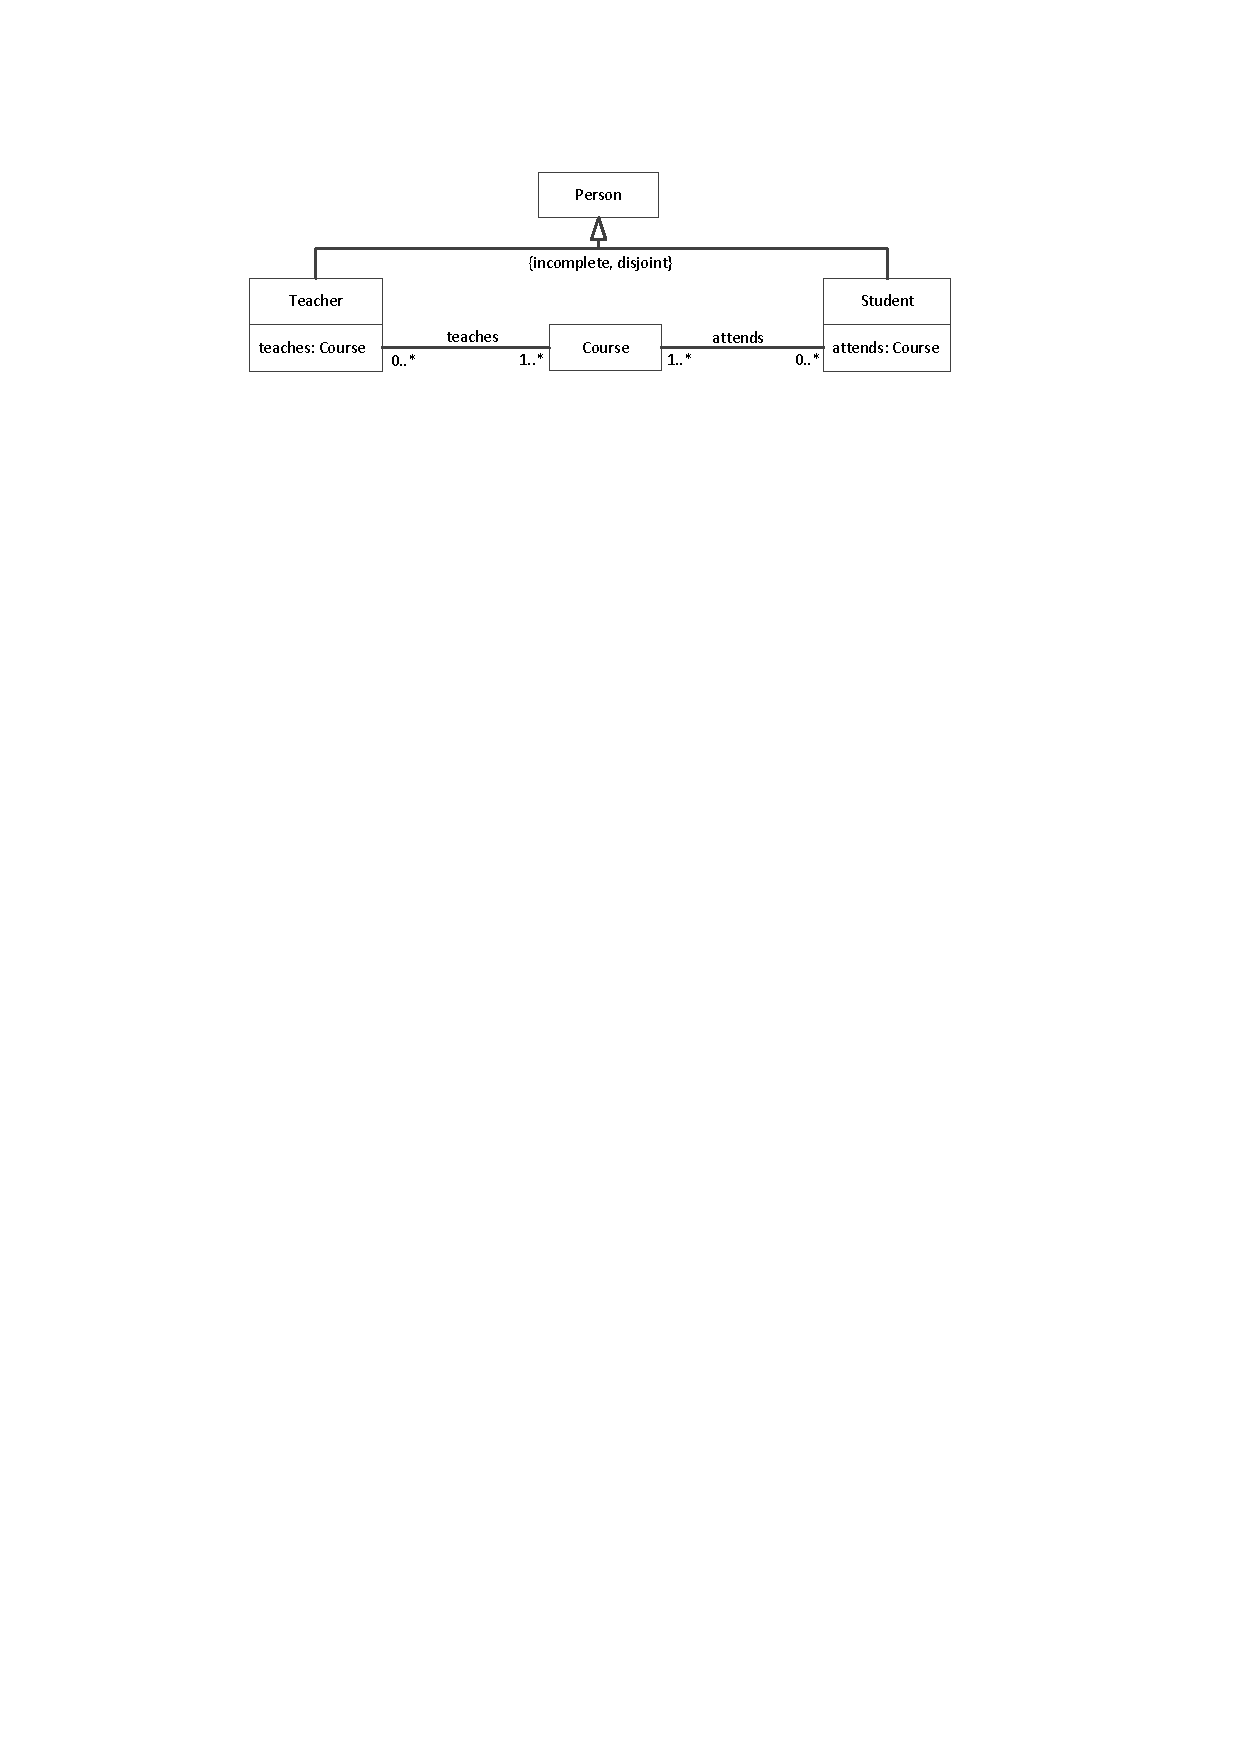
\includegraphics[trim = 40mm 230mm 45mm 25mm, clip, scale=0.9]{./UniversityClassDiagram0Simplified.pdf}
    \caption{An example UML class diagram}\label{fig_UniversityClassDiagram0}
    \end{figure}  
   
   
   We assume we start with the UML class diagram of Figure~\ref{fig_UniversityClassDiagram0}.
   We highlight a few key points of  Figure~\ref{fig_UniversityClassDiagram0} as a means to briefly describe UML notation that are of relevance for this sequel.   It states that $\mathsf{Person}$, $\mathsf{Student}$ and $\mathsf{Teacher}$ are in an \textbf{inheritance hierarchy} where $\mathsf{Student}$ and $\mathsf{Teacher}$ are \textbf{subclasses} of the $\mathsf{Person}$ class. $\mathsf{incomplete}$ in the $\{\mathsf{incomplete, disjoint}\}$ annotation states explicitly that there are instances that are instances of  the $\mathsf{Person}$ class, but that are not instances of the $\mathsf{Student}$ class, nor are they instances of the $\mathsf{Teacher}$ class. $\mathsf{disjoint}$ stipulates that $\mathsf{Student}$ and $\mathsf{Teacher}$ classes  do not share any instances. 

       More generally an inheritance hierarchy can be annotated with a $\{\mathsf{covering, disjoint}\}$ annotation. Permitted values for $\mathsf{covering}$ are $\mathsf{complete}$ and $\mathsf{incomplete}$ where $\mathsf{complete}$ indicates that  every instance of the parent class is also an instance of at least one child class and $\mathsf{incomplete}$ indicates that every instance of the parent class is not necessarily an instance of a child class.  That is, there are instances of the parent class that are not specialized by a child class.  $\mathsf{disjoint}$ indicates whether an instance can belong to more than one child class.  Permitted values for $\mathsf{disjoint}$ are $\mathsf{overlapping}$ and $\mathsf{disjoint}$. $\mathsf{overlapping}$ indicates that an instance can belong to more than one child class while $\mathsf{disjoint}$ states  that an instance can at most belong to one child class. When an inheritance hierarchy is not explicitly annotated with a $\{\mathsf{covering, disjoint}\}$ annotation, the default annotation $\{\mathsf{incomplete, disjoint}\}$ is assumed to apply~\cite{UML2.5.1}. 
     
     Figure~\ref{fig_UniversityClassDiagram0} indicates that a $\mathsf{teaches}$ \textbf{association} exists between $\mathsf{Teacher}$ and $\mathsf{Course}$. The $1..*$ multiplicity stipulates that a teacher teaches one or more courses, while $0..*$ states that a course is taught by zero (indicates a course that must completed through self-study) or more teachers. The $\mathsf{attends}$ association states that students have to attend one or more courses and a course may be attended by zero (i.e. no students are enrolled for the course) or more students. 
     
     The corresponding TBox definition for Figure~\ref{fig_UniversityClassDiagram0} is:
     
   \begin{align}
  \mathcal{T}_0^{UML} = \{\mathsf{Course} &\sqsubseteq \neg \mathsf{Person},\\
  \mathsf{Teacher} &\sqsubseteq \mathsf{Person}, \\
  \mathsf{Teacher} &\sqsubseteq \exists \mathsf{teaches}.\top, \\
  \exists\mathsf{teaches}.\top &\sqsubseteq \mathsf{Teacher}, \\
  \top &\sqsubseteq \forall \mathsf{teaches}.\mathsf{Course}, \\
  \mathsf{Student} &\sqsubseteq \mathsf{Person},\\
  \mathsf{Student} &\sqsubseteq \exists \mathsf{attends}.\top, \\
  \exists\mathsf{attends}.\top &\sqsubseteq \mathsf{Student}, \\
  \top &\sqsubseteq \forall \mathsf{attends}.\mathsf{Course}, \\
  \mathsf{Student} &\sqsubseteq \neg \mathsf{Teacher}\}
  \end{align}   
  
  The meaning of these axioms are as follows:
  \begin{enumerate}
  	\item Persons and courses are disjoint.
  	\item Teachers are a subset of persons.
  	\item Teachers teach at least one course.
  	\item The domain of $\mathsf{teaches}$ is $\mathsf{Teacher}$.
  	\item The range of $\mathsf{teaches}$ is $\mathsf{Course}$.
  	\item Students are a subset of persons.
  	\item Students attend at least one course.
  	\item The domain of $\mathsf{attends}$ is $\mathsf{Student}$.
	\item The range of $\mathsf{attends}$ is $\mathsf{Course}$. 
	\item Students and teachers are disjoint.
  \end{enumerate}


   
    \subsection{Analysis of a UML Class Diagram using Armstrong ABoxes for $\mathcal{ALC}$ TBoxes}
    In this section we illustrate the analysis of a UML class diagram for the $\mathsf{Person}$ class of Figure~\ref{fig_UniversityClassDiagram0} using Armstrong ABoxes.  We start our analysis by generating an Armstrong object diagram for $\mathsf{Person}$ and its siblings. Since $\mathsf{Person}$ is a top level class (i.e. it has no superclass/parent), we consider all top level classes in Figure~\ref{fig_UniversityClassDiagram0}. Hence, we generate an Armstrong ABox for $\mathcal{T}_0^{UML}$ and $M = \{\mathsf{Person}, \mathsf{Course}\}$. This Armstrong ABox be will the same as the one represented in Table~\ref{tab_ArmstrongABox_Person_Course}, for which the corresponding Armstrong object diagram is given in Figure~\ref{fig_ArmstrongOD_Person_Course}. 
    
    
    The object diagram is enriched with constraints expressed in Object Constraint Language (OCL)~\cite{OCL2.4}. In representing an Armstrong ABox as an object diagram we are forced to use OCL for four reasons.
    \begin{itemize}
     \item It is not possible to express in an object diagram that an instance must be of a type that is the union of two or more classes. In particular to express that $x_1$ is an instance of the union of $\mathsf{Person}$ and $\mathsf{Course}$ we state that for $x_1$ the invariant 
     \[\mathsf{oclIsTypeOf}(\mathsf{Person}) \hspace{5pt} \mathsf{or} \hspace{5pt} \mathsf{oclIsTypeOf}(\mathsf{Person})\] 
     holds. 
     \item It is not possible to express  negative information in an object diagram. In particular to express that $x_2$ is not an instance of the $\mathsf{Person}$ class we add the invariant 
     \[\mathsf{not} \hspace{5pt} \mathsf{oclIsTypeOf}(\mathsf{Person}).\]
     \item It is not possible to express implication in an object diagram. In general satisfying exemplars state that when an individual $x$ is of a given type, say $\mathsf{A}$, it implies that it must also be an individual of another type, say $\mathsf{B}$. In OCL this can be expressed as 
     \[\mathsf{oclIsTypeOf}(\mathsf{A}) \hspace{5pt} \mathsf{implies} \hspace{5pt} \mathsf{oclIsTypeOf}(\mathsf{B}),\]
     assuming that instance $x$ is the context of the OCL expression.
     \item For each instance we want to indicate whether it serves as a satisfying- or violating exemplar. For this purpose we introduce the $<<\mathsf{Satisfying \hspace{1mm} exemplar}>>$ and \\$<<\mathsf{Violating \hspace{1mm} exemplar}>>$ stereotypes~\cite{UML2.5.1}.
    \end{itemize}

    Similar to Table~\ref{tab_ArmstrongABox_Person_Course}, Figure~\ref{fig_ArmstrongOD_Person_Course} depicts three instances, $x_1$, $x_2$ and $x_3$. For each instance type information is provided in a combination of graphical notation and OCL constraint. The context of an OCL constraint is given by the dashed line linking an OCL contraint with a particular instance.  Each of the three instances represent violating exemplars.
    \begin{description}
     \item[$x_1$] All type information is expressed as an OCL constraint.
     \item[$x_2$] The graphical notation stipulates that $x_2$ is of type $\mathsf{Course}$ and the OCL constraint further stipulates that $x_2$ is not an instance of the $\mathsf{Person}$ class.  Hence, both these conditions must hold for $x_2$.
     \item[$x_3$] The graphical notation stipulates that $x_3$ is of type $\mathsf{Person}$ and the OCL constraint further stipulates that $x_3$ is not an instance of the $\mathsf{Course}$ class.     
    \end{description} 
   
    
    \begin{figure}
    %trim option's parameter order: left bottom right top
    \centering 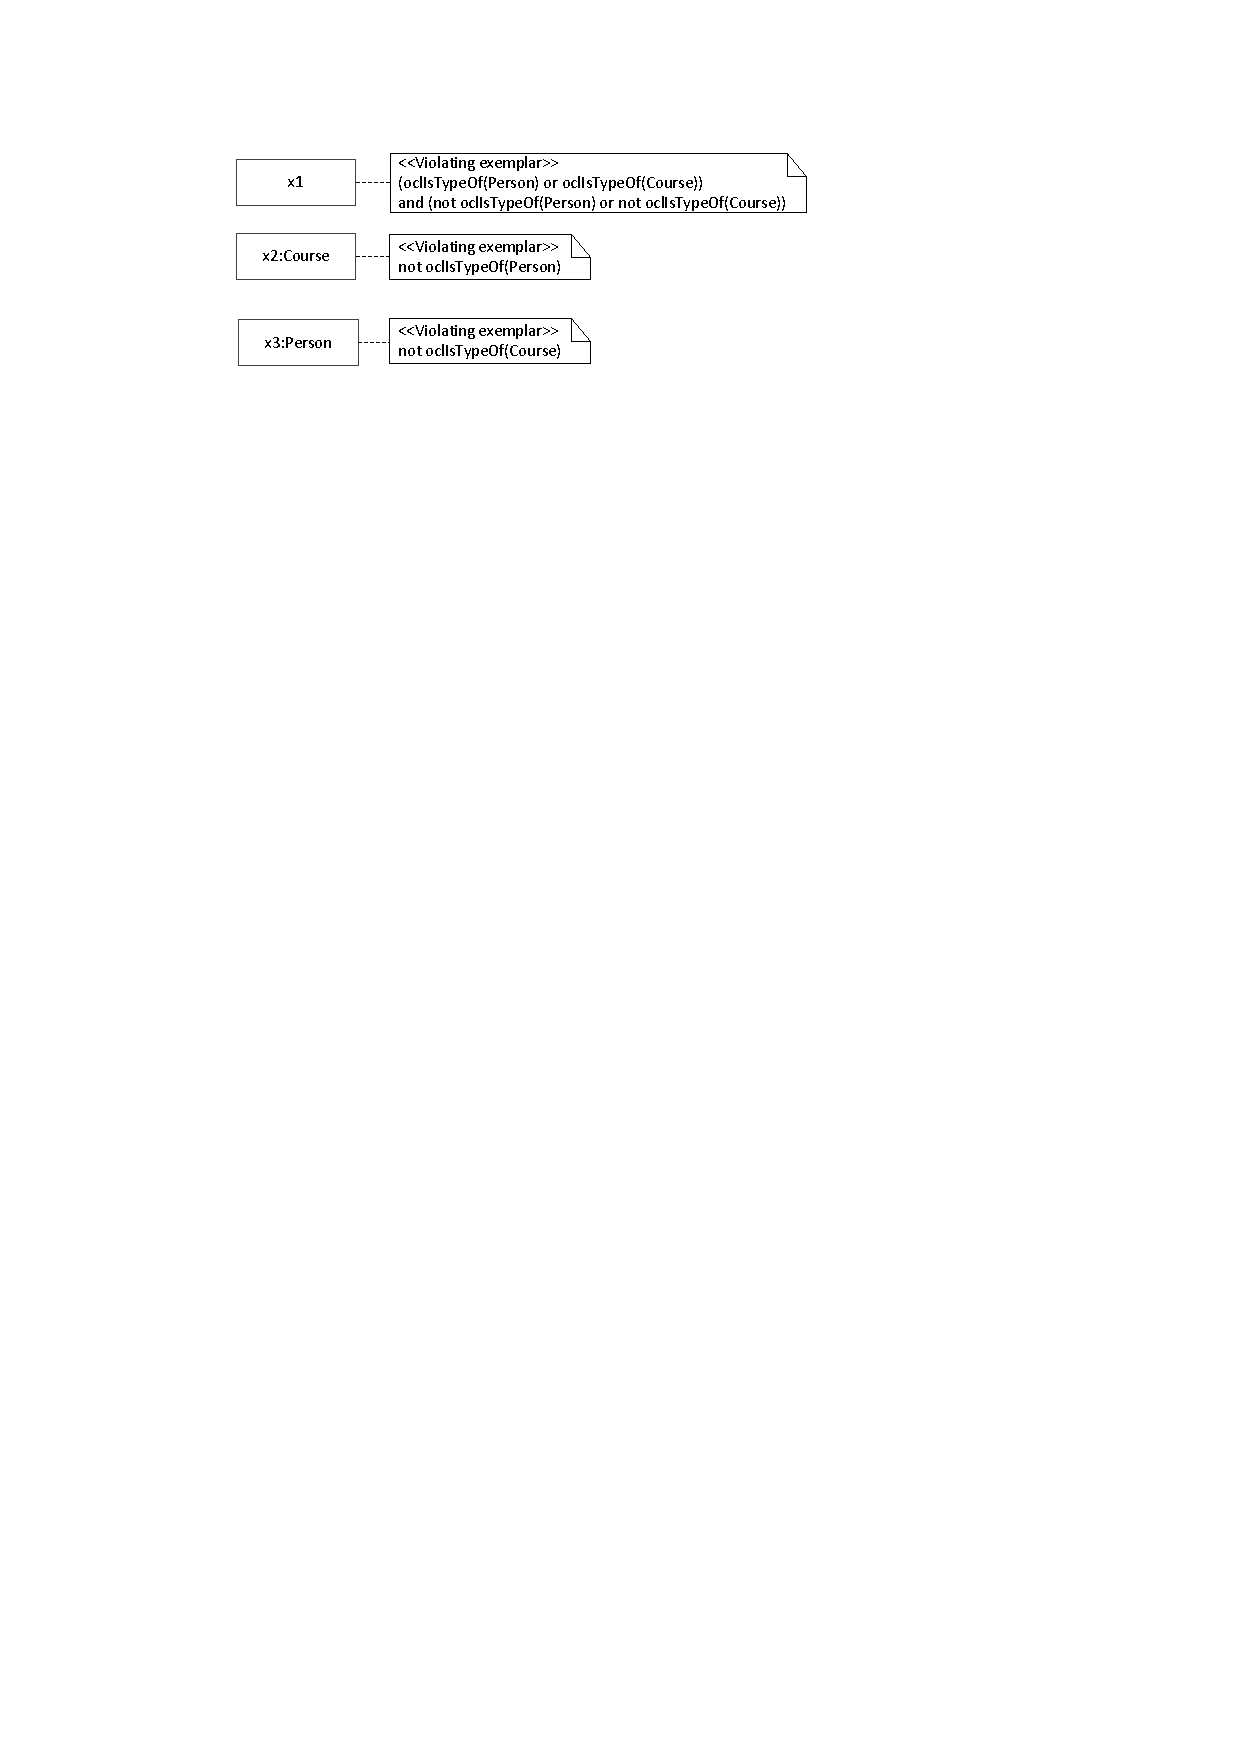
\includegraphics[trim = 30mm 234mm 55mm 25mm, clip, scale=0.9]{./ArmstrongOD_Person_Course.pdf}
    \caption{Armstrong object diagram corresponding to Table~\ref{tab_ArmstrongABox_Person_Course}}\label{fig_ArmstrongOD_Person_Course}
    \end{figure}   

    
     To analyse how the $\mathsf{Person}$ class relates to its direct subclasses/children, we generate an Armstrong object diagram for the UML class diagram of Figure~\ref{fig_UniversityClassDiagram0} and $M = \{\mathsf{Person}, \mathsf{Student} \sqcup \mathsf{Teacher}\}$. Hence, an Armstrong ABox is generated for $\mathcal{T}_0^{UML}$ and $M = \{\mathsf{Person}, \mathsf{Student} \sqcup \mathsf{Teacher}\}$. This Armstrong ABox is similar to the one illustrated in Table~\ref{tab_ArmstrongABox_Person_StudentORTeacher}, for which the Armstrong object diagram is given in Figure~\ref{fig_ArmstrongOD_Person_StudentORTeacher}. 
     
     Again, if we assume our application domain deals only with persons that are students and/or teachers, the $x_1$ instance does not capture a scenario that is possible in our application domain. To address this we need to amend our class diagram with a $\{\mathsf{complete}, \mathsf{disjoint}\}$ annotation for the inheritance hierarchy consisting of $\mathsf{Person}$ with subclasses $\mathsf{Student}$ and $\mathsf{Teacher}$.  This is illustrated in Figure~\ref{fig_UniversityClassDiagram1}, which corresponds with $\mathcal{T}_1^{UML}$. The revised Armstrong object diagram is given in Figure~\ref{fig_ArmstrongOD_Person_StudentORTeacher_Revised} which corresponds to Table~\ref{tab_ArmstrongABox_Person_StudentORTeacher_Revised}.
     
    \begin{align*}
	\mathcal{T}_1^{UML} = \{\mathsf{Course} &\sqsubseteq \neg \mathsf{Person},\\
	\mathsf{Person} &\equiv \mathsf{Student} \sqcup \mathsf{Teacher}, \\   
    \mathsf{Teacher} &\sqsubseteq \mathsf{Person}, \\
	\mathsf{Teacher} &\sqsubseteq \exists \mathsf{teaches}.\top, \\
	\exists\mathsf{teaches}.\top &\sqsubseteq \mathsf{Teacher}, \\
	\top &\sqsubseteq \forall \mathsf{teaches}.\mathsf{Course}, \\
	\mathsf{Student} &\sqsubseteq \mathsf{Person},\\
	\mathsf{Student} &\sqsubseteq \exists \mathsf{attends}.\top, \\
	\exists\mathsf{attends}.\top &\sqsubseteq \mathsf{Student}, \\
	\top &\sqsubseteq \forall \mathsf{attends}.\mathsf{Course}, \\
	\mathsf{Student} &\sqsubseteq \neg \mathsf{Teacher}\}
   \end{align*}     
     
    \begin{figure}
    %trim option's parameter order: left bottom right top
    \centering 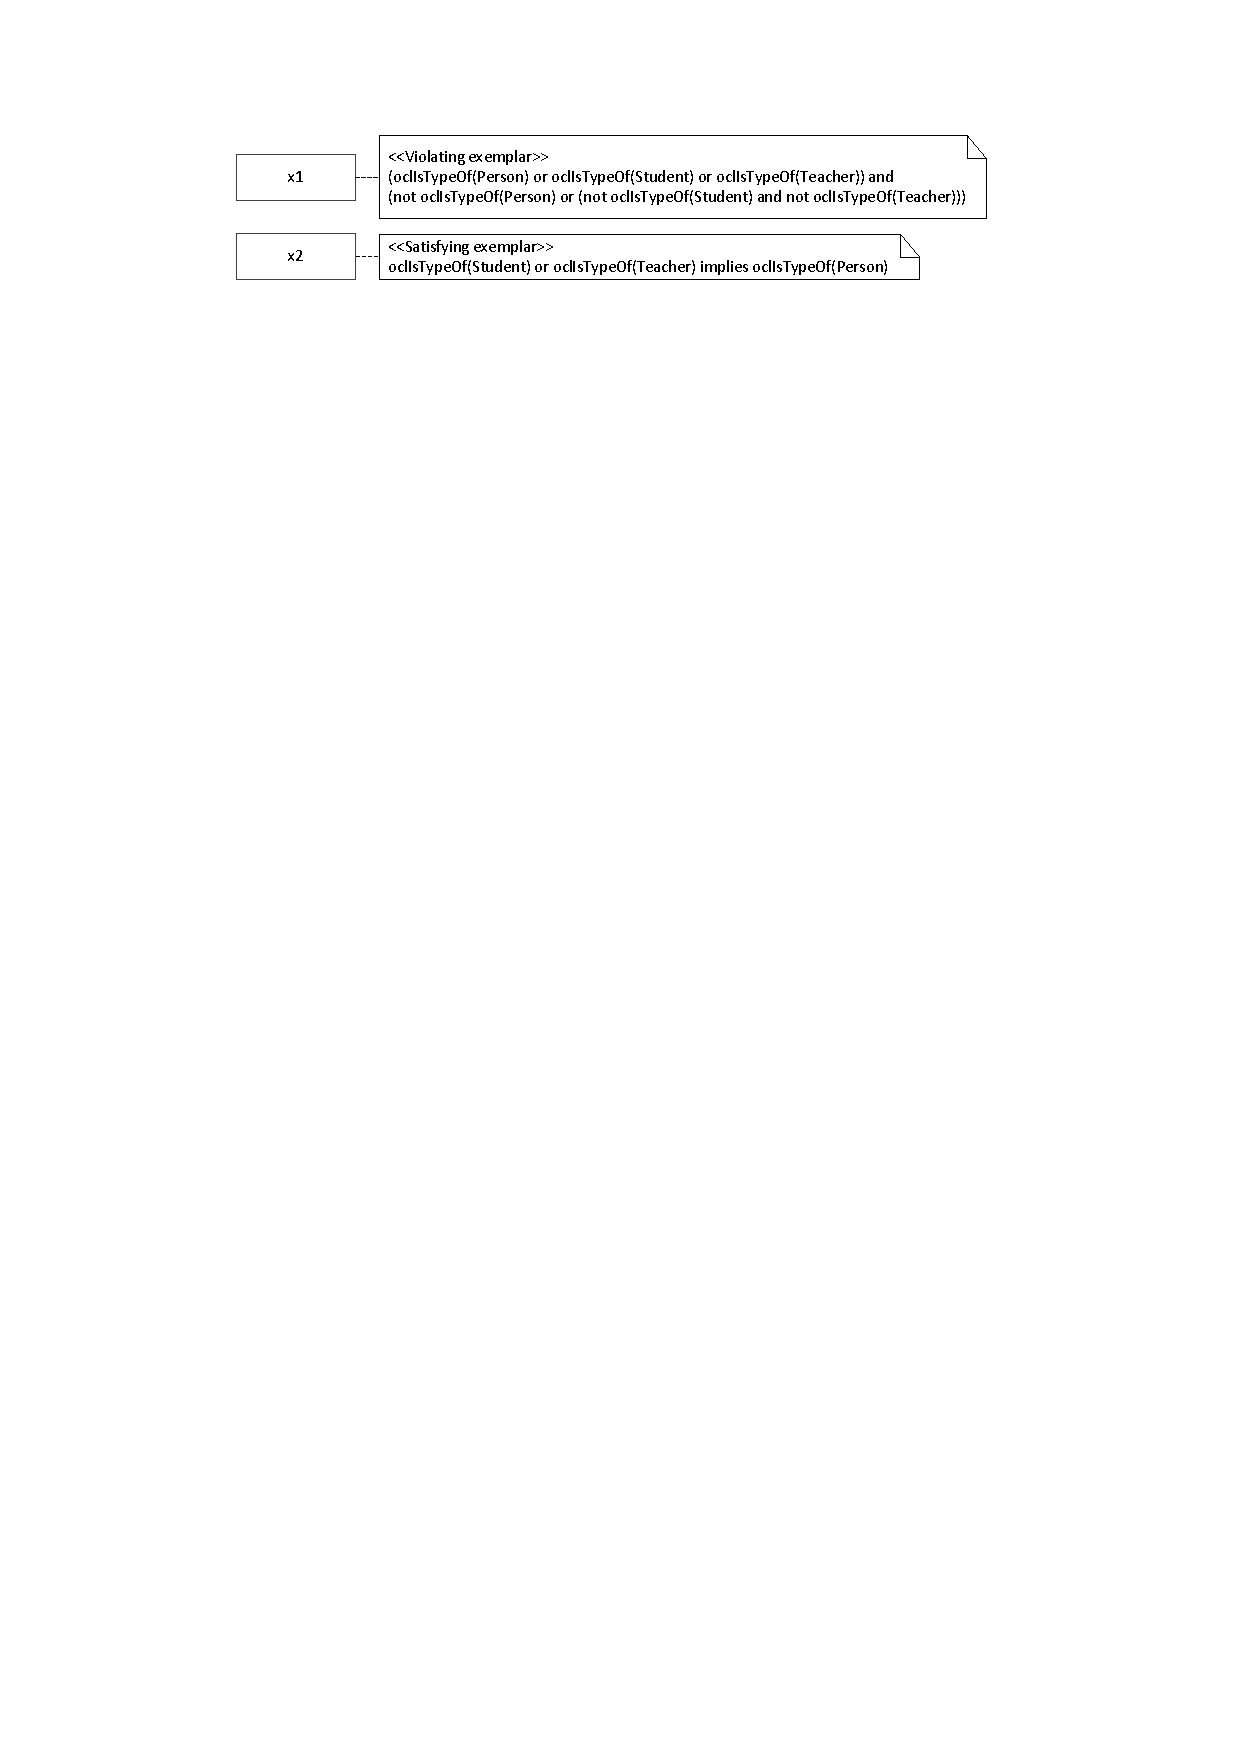
\includegraphics[trim = 20mm 245mm 0mm 20mm, clip, scale=0.9]{./ArmstrongOD_Person_StudentORTeacher.pdf}
    \caption{Armstrong object diagram corresponding to Table~\ref{tab_ArmstrongABox_Person_StudentORTeacher}}\label{fig_ArmstrongOD_Person_StudentORTeacher}
    \end{figure} 
    
    \begin{figure}
    %trim option's parameter order: left bottom right top
    \centering 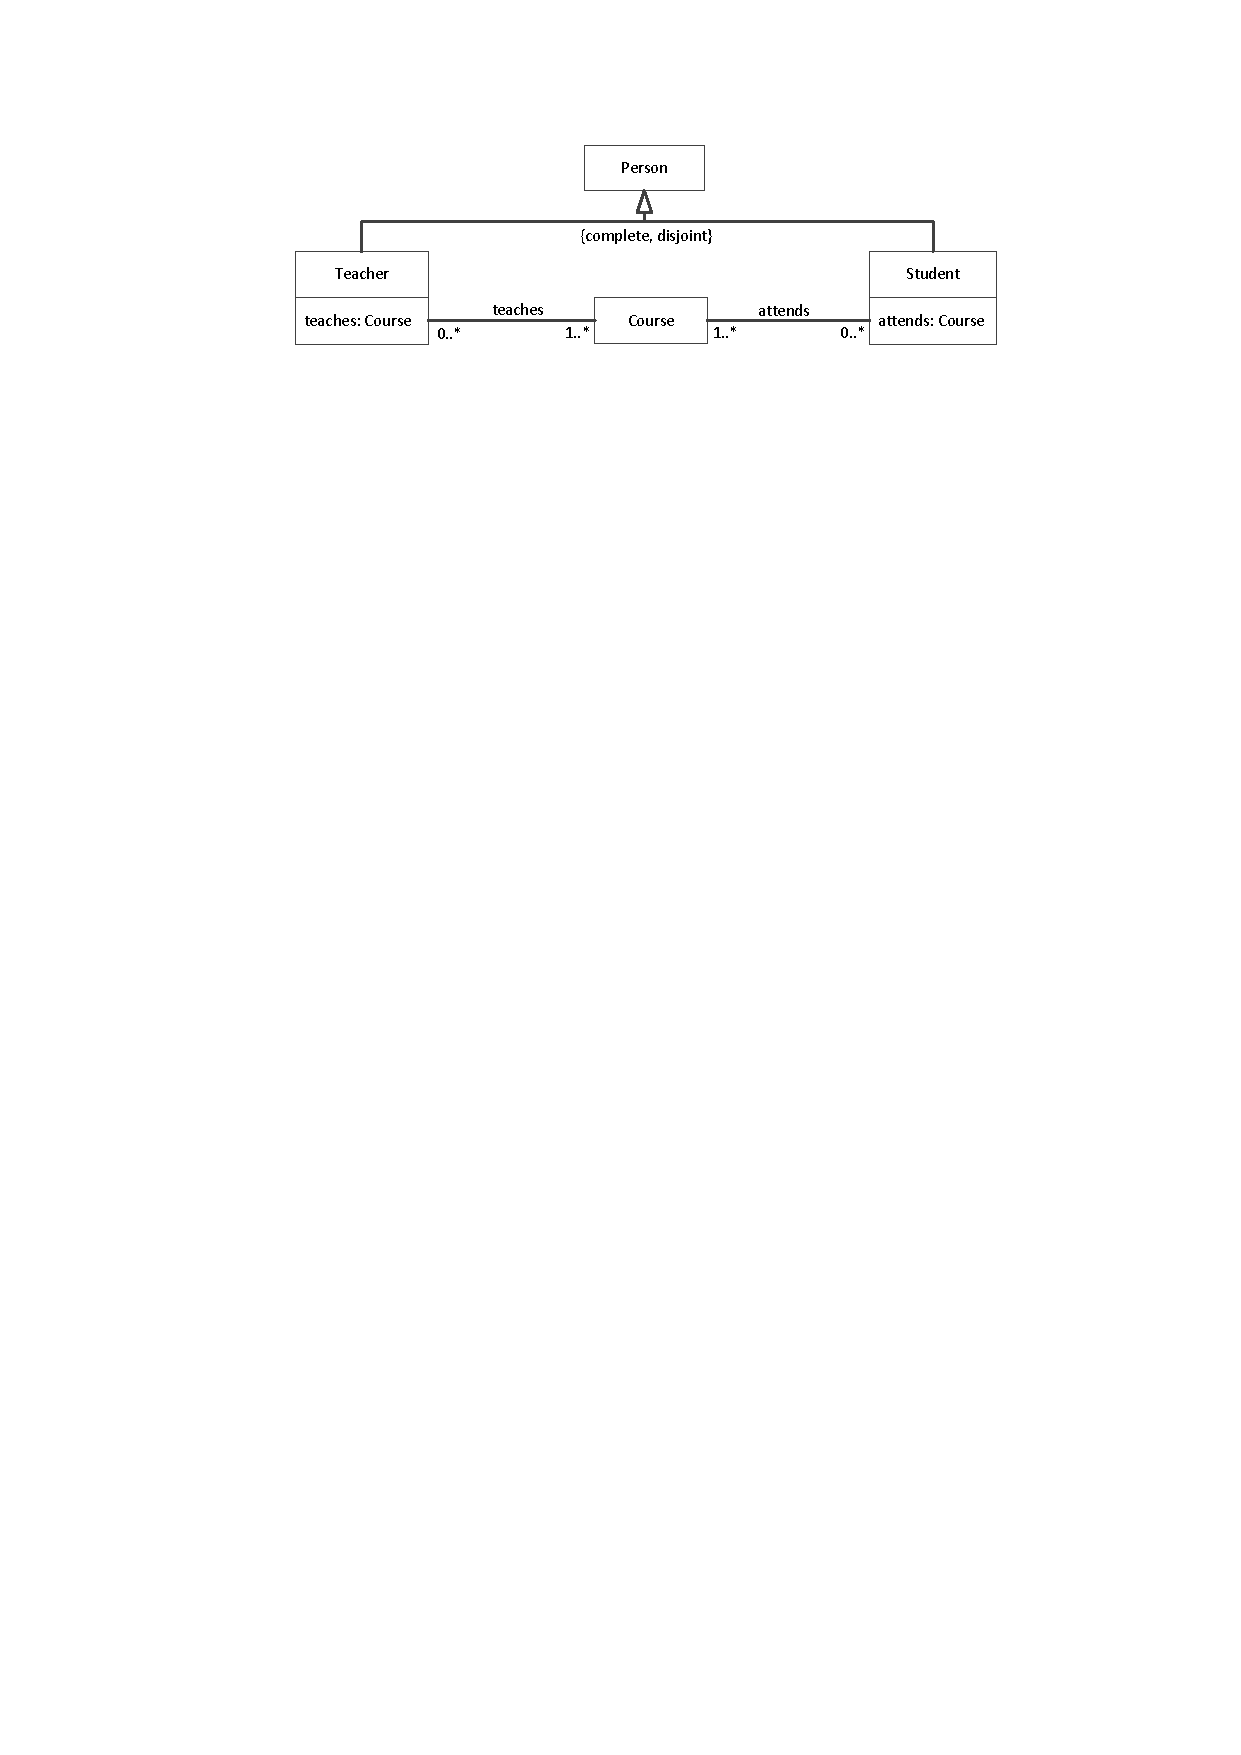
\includegraphics[trim = 40mm 235mm 30mm 20mm, clip, scale=0.9]{./UniversityClassDiagram1Simplified.pdf}
    \caption{All instances of $\mathsf{Person}$ are either instances of $\mathsf{Student}$ or $\mathsf{Teacher}$}\label{fig_UniversityClassDiagram1}
    \end{figure}   
        
          \rowcolors{1}{white}{lightgray}
   \begin{table}
   \footnotesize
 %     \scriptsize
     \begin{center} 
       \caption{Armstrong ABox for $\mathcal{T}_1^{UML}$ and $M=\{\mathsf{Person}, \mathsf{Student} \sqcap \mathsf{Teacher}\}$}
       \label{tab_ArmstrongOD_Person_StudentANDTeacher}
       \smallskip
       \begin{tabular}
       {|>{\footnotesize}p{\tableEntailmentSpacing}|>{\footnotesize}p{\tableExamplarSpacing}|>{\footnotesize}p{\tableExamplarSpacing}|>{\footnotesize}p{\tableCommentSpacing}|}
       \hline
        \multicolumn{1}{|>{\footnotesize}c|}{\textbf{Non-Entailment}}&\multicolumn{2}{>{\footnotesize}c|}{\textbf{Violating exemplar}}&\multicolumn{1}{>{\footnotesize}c|}{\textbf{Comment}}\\
        \hline
        \begin{minipage}{\tableEntailmentSpacing}
        \vspace{2pt}
            $\begin{aligned}
              &\mathsf{Person} \hspace{2pt}\sqcup \\
              &\hspace{\tableEquationIndent}(\mathsf{Student} \sqcap \mathsf{Teacher})\\
  	      &\sqsubseteq\\
  	      &\mathsf{Person} \hspace{2pt} \sqcap \\
  	      &\hspace{\tableEquationIndent}(\mathsf{Student} \sqcap \mathsf{Teacher})\\
           \end{aligned}$
  	\end{minipage}
        &
        \begin{minipage}{\tableExamplarSpacing}
  	    $\begin{aligned}
               &(\mathsf{Person} \hspace{2pt}\sqcup \\
              &\hspace{\tableEquationIndent}(\mathsf{Student} \sqcap \mathsf{Teacher}))(x_1)
  	    \end{aligned}$
  	\end{minipage}
  	&
  	\begin{minipage}{\tableExamplarSpacing}
  	    \vspace{2pt}
  	   $\begin{aligned}
             &\neg(\mathsf{Person} \hspace{2pt} \sqcap \\
  	      &\hspace{\tableEquationIndent}(\mathsf{Student} \sqcap \mathsf{Teacher}))(x_1)
  	    \end{aligned}$ 
  	\end{minipage}
        &
        \begin{minipage}{\tableCommentSpacing}
            \vspace{2pt}
           It is possible that there are individuals that are persons or that are students and teachers, but that are not persons, or they are not students, or they are not teachers. This is true since there are students that are not teachers.
            \vspace{2pt}
        \end{minipage}     
        \\    
        \begin{minipage}{\tableEntailmentSpacing}
        \vspace{2pt}
            $\begin{aligned}
              &\mathsf{Person} \hspace{2pt} \\
  	      &\sqsubseteq\\
              &\mathsf{Student} \sqcap \mathsf{Teacher}
            \end{aligned}$
  	\end{minipage}
        &
        \begin{minipage}{\tableExamplarSpacing}
  	    $\begin{aligned}
               &\mathsf{Person}(x_2)
  	    \end{aligned}$
  	\end{minipage}
  	&
  	\begin{minipage}{\tableExamplarSpacing}
  	    \vspace{2pt}
  	   $\begin{aligned}
             &\neg(\mathsf{Student} \sqcap \mathsf{Teacher})(x_2)
  	    \end{aligned}$ 
  	\end{minipage}
        &
        \begin{minipage}{\tableCommentSpacing}
            \vspace{2pt}
           It is possible that individuals that are persons are either not students or not teachers, which is correct.
            \vspace{2pt}
        \end{minipage}     
        \\        
        \hline
       \end{tabular}
     \end{center}
     \normalsize
   \end{table} 
   
    \begin{figure}
    %trim option's parameter order: left bottom right top
    \centering 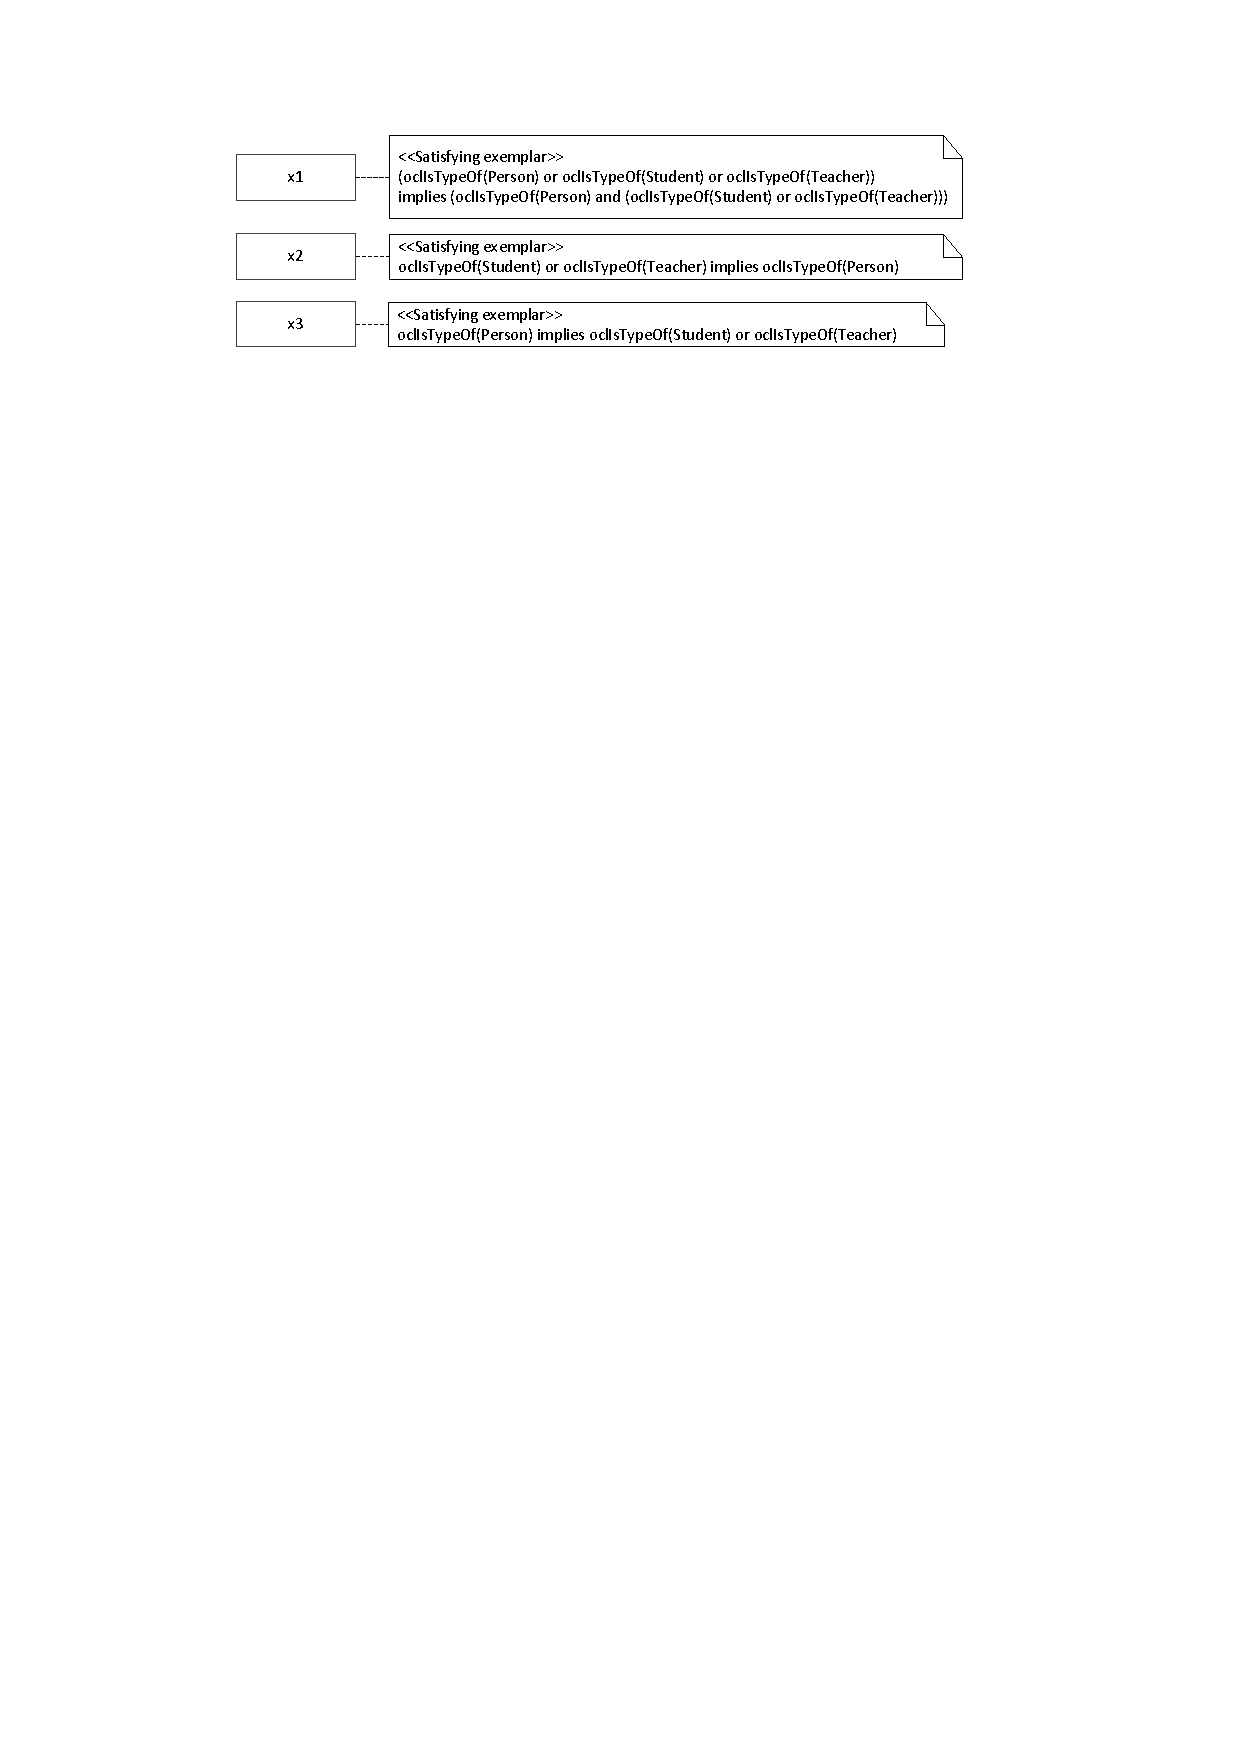
\includegraphics[trim = 20mm 235mm 42mm 20mm, clip, scale=0.9]{./ArmstrongOD_Person_StudentORTeacher_Revised.pdf}
    \caption{Armstrong object diagram corresponding to Table~\ref{tab_ArmstrongABox_Person_StudentORTeacher_Revised}}\label{fig_ArmstrongOD_Person_StudentORTeacher_Revised}
    \end{figure}      
   
    
        \begin{figure}
    %trim option's parameter order: left bottom right top
    \centering 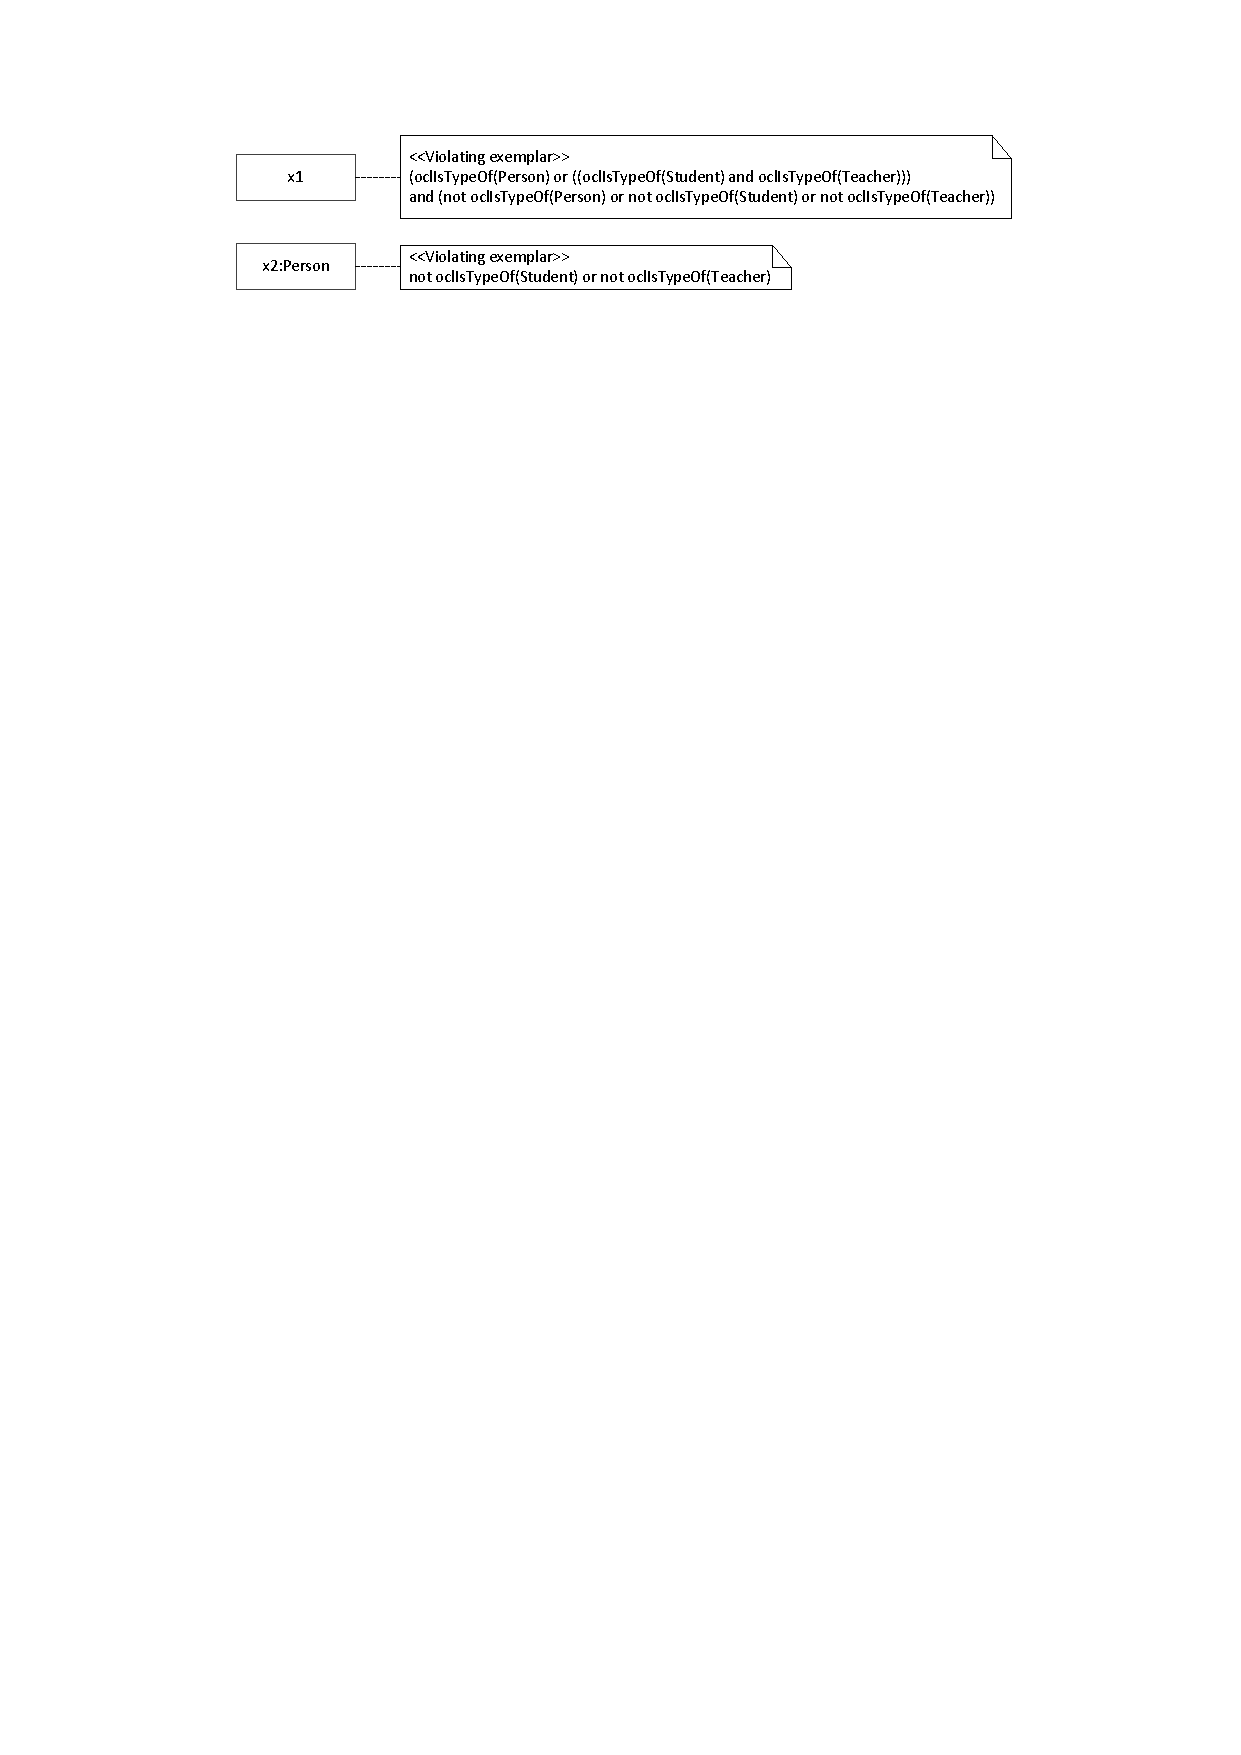
\includegraphics[trim = 30mm 245mm 30mm 20mm, clip, scale=0.9]{./ArmstrongOD_Person_StudentANDTeacher.pdf}
    \caption{Armstrong object diagram corresponding to Table~\ref{tab_ArmstrongOD_Person_StudentANDTeacher}}\label{fig_ArmstrongOD_Person_StudentANDTeacher}
    \end{figure} 
   
       To further investigate how the $\mathsf{Person}$ class relates to its direct subclasses, we generate an Armstrong object diagram for the UML class diagram of Figure~\ref{fig_UniversityClassDiagram0} and $M = \{\mathsf{Person}, \mathsf{Student} \sqcap \mathsf{Teacher}\}$.
      This Armstrong ABox is represented in Table~\ref{tab_ArmstrongOD_Person_StudentANDTeacher}, for which the Armstrong object diagram is given in Figure~\ref{fig_ArmstrongOD_Person_StudentANDTeacher}. Even though both violating exemplars describe our application domain accurately, this Armstrong ABox/Armstrong object diagram does not describe our application accurately. What is missing is a satisfying exemplar stating that an individual that is both a student and a teacher, is necessarily a person, similar to the satisfying exemplar defined by $x_2$ in Table~\ref{tab_ArmstrongABox_Person_StudentANDTeacher}. Why is this satisfying exemplar missing from Table~\ref{tab_ArmstrongOD_Person_StudentANDTeacher} and Figure~\ref{fig_ArmstrongOD_Person_StudentANDTeacher}? It is missing because $\mathsf{Student} \sqcap \mathsf{Teacher} \sqsubseteq \mathsf{Person}$ is not an entailment that follows from $\mathcal{T}_1^{UML}$ due to the axiom $\mathsf{Student} \sqsubseteq \neg \mathsf{Teacher}$. This axiom states explicitly that $\mathsf{Student}$ is disjoint from $\mathsf{Teacher}$. This disjointness originates from the $\{\mathsf{complete}, \mathsf{disjoint}\}$ annotation of the $\mathsf{Person}$ hierarchy of the UML class diagram.    

       To allow for the possibility where a teacher can be a student as well, we revise the $\{\mathsf{complete}, \mathsf{disjoint}\}$ annotation of the $\mathsf{Person}$ hierarchy to be $\{\mathsf{complete}, \mathsf{overlapping}\}$. This is illustrated in Figure~\ref{fig_UniversityClassDiagram2}, for which the related translation to $\mathcal{ALC}$ is given by $\mathcal{T}_2^{UML}$. If we now generate an Armstrong ABox for $\mathsf{T}_2^{UML}$ and $M = \{\mathsf{Person}, \mathsf{Student} \sqcap \mathsf{Teacher}\}$, it generates an Armstrong ABox similar to that of Table~\ref{tab_ArmstrongABox_Person_StudentANDTeacher}, for which a related Armstrong object diagram can be created.


     \begin{figure}
    %trim option's parameter order: left bottom right top
    \centering 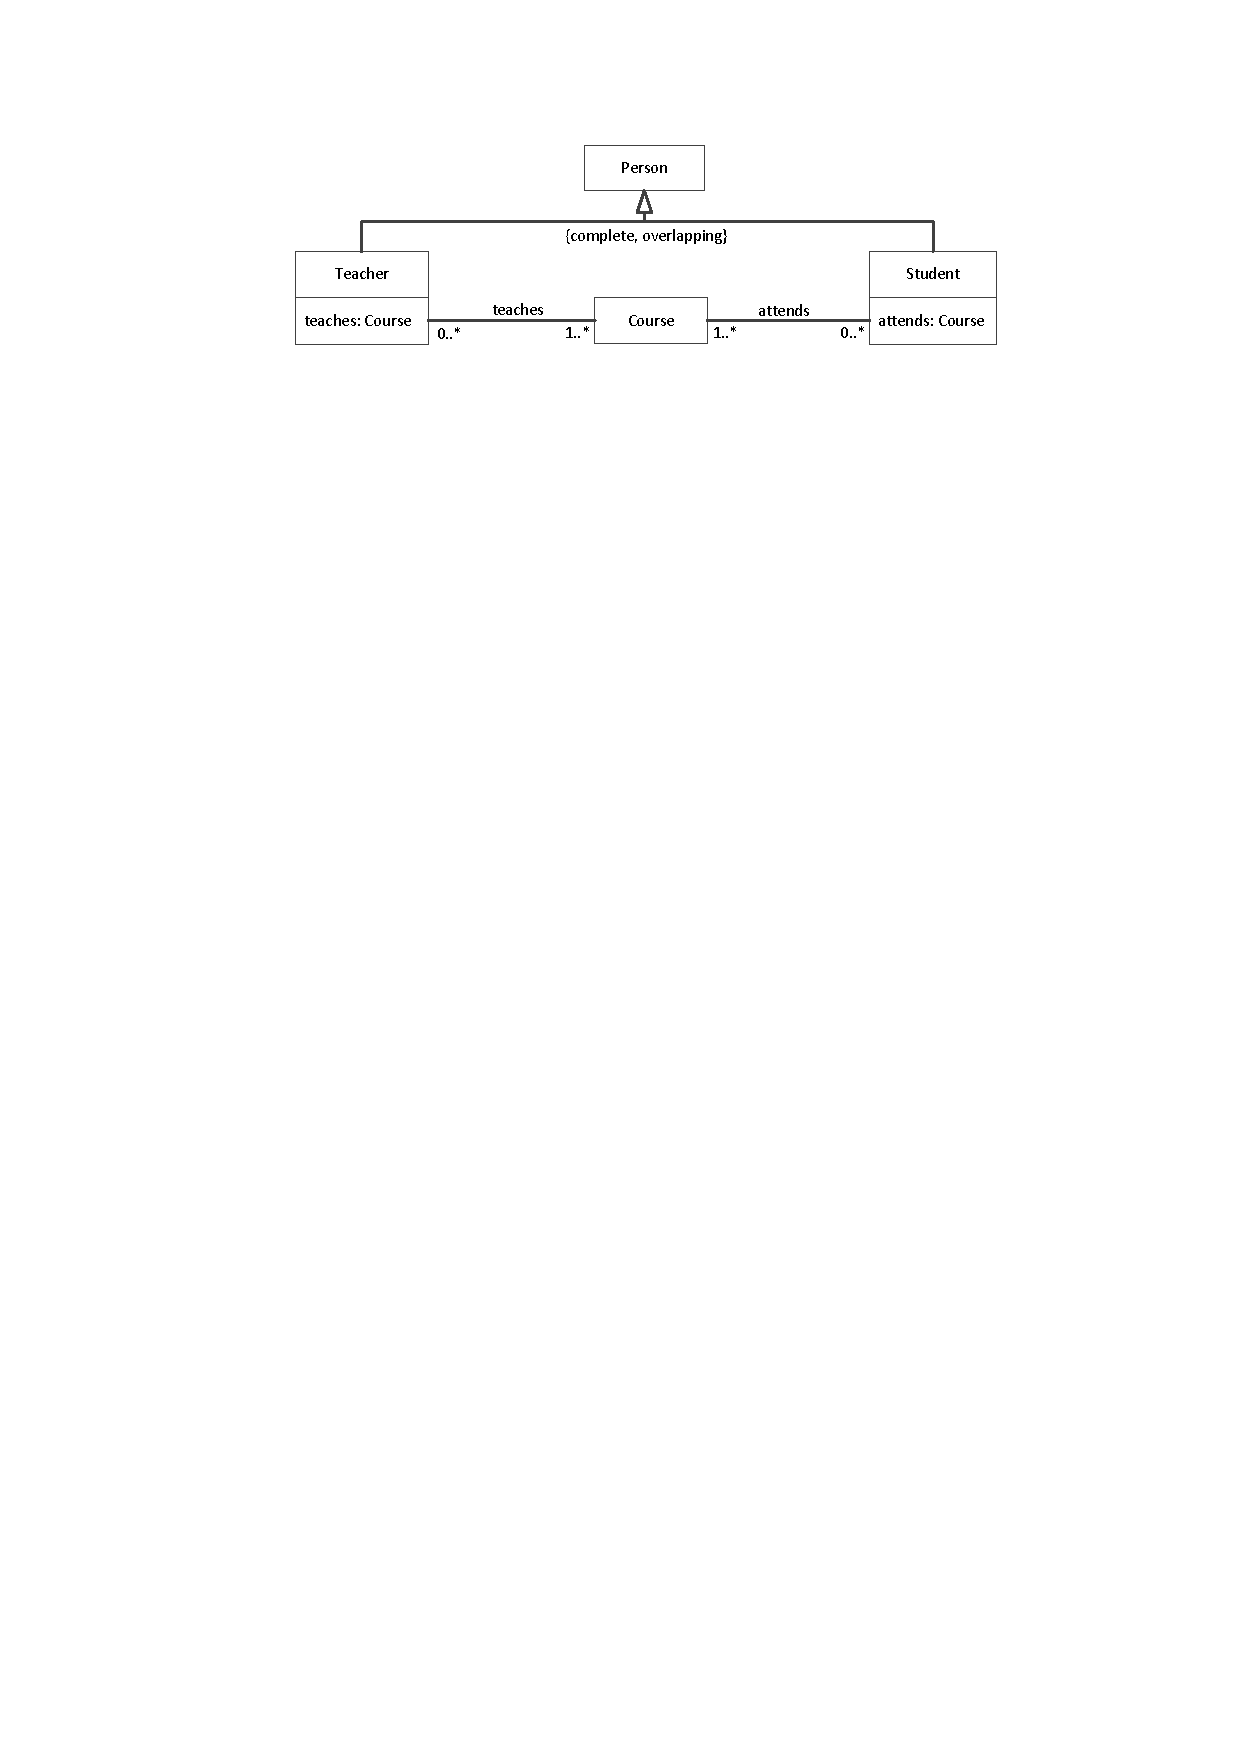
\includegraphics[trim = 40mm 235mm 30mm 20mm, clip, scale=0.9]{./UniversityClassDiagram2Simplified.pdf}
    \caption{Teachers can be students as well}\label{fig_UniversityClassDiagram2}
    \end{figure}  

    
     \begin{align*}
	\mathcal{T}_1^{UML} = \{\mathsf{Course} &\sqsubseteq \neg \mathsf{Person},\\
	\mathsf{Person} &\equiv \mathsf{Student} \sqcup \mathsf{Teacher}, \\   
	\mathsf{Teacher} &\sqsubseteq \mathsf{Person}, \\
	\mathsf{Teacher} &\sqsubseteq \exists \mathsf{teaches}.\top, \\
	\exists\mathsf{teaches}.\top &\sqsubseteq \mathsf{Teacher}, \\
	\top &\sqsubseteq \forall \mathsf{teaches}.\mathsf{Course}, \\
	\mathsf{Student} &\sqsubseteq \mathsf{Person},\\
	\mathsf{Student} &\sqsubseteq \exists \mathsf{attends}.\top, \\
	\exists\mathsf{attends}.\top &\sqsubseteq \mathsf{Student}, \\
	\top &\sqsubseteq \forall \mathsf{attends}.\mathsf{Course}\} 
  \end{align*}     
 
   To investigate how students and teachers relate to each other, we can generate an Armstrong ABox for $\mathcal{T}_2^{UML}$ and $M = \{\mathsf{Student}, \mathsf{Teacher}\}$, which will result in an Armstrong ABox similar to that given in Table~\ref{tab_ArmstrongABox_Student_Teacher}. This Armstrong ABox provides no basis for changes to the UML class diagram of Figure~\ref{fig_UniversityClassDiagram2}.
   
 
          \rowcolors{1}{white}{lightgray}
   \begin{table}
   \footnotesize
 %     \scriptsize
     \begin{center} 
       \caption{Armstrong ABox for $\mathcal{T}_2^{UML}$ and $M=\{\mathsf{Student}, \exists\mathsf{attends}.\top\}$}
       \label{tab_ArmstrongOD_Student_AttendsSomeThing}
       \smallskip
       \begin{tabular}
       {|>{\footnotesize}p{\tableEntailmentSpacing}|>{\footnotesize}p{\tableExamplarSpacing}|>{\footnotesize}p{\tableExamplarSpacing}|>{\footnotesize}p{\tableCommentSpacing}|}
       \hline
        \multicolumn{1}{|>{\footnotesize}c|}{\textbf{Entailment}}&\multicolumn{2}{>{\footnotesize}c|}{\textbf{Satisfying exemplar}}&\multicolumn{1}{>{\footnotesize}c|}{\textbf{Comment}}\\
        \hline
        \begin{minipage}{\tableEntailmentSpacing}
        \vspace{2pt}
         $\begin{aligned}
          &\mathsf{Student} \hspace{2pt}\sqcup \\
          &\hspace{\tableEquationIndent}\exists \mathsf{attends}.\top\\
  	      &\sqsubseteq\\
  	      &\mathsf{Student} \hspace{2pt} \sqcap \\
  	      &\hspace{\tableEquationIndent}\exists \mathsf{attends}.\top\\
           \end{aligned}$
  	\end{minipage}
        &
        \begin{minipage}{\tableExamplarSpacing}
  	    $\begin{aligned}
               &(\mathsf{Student} \hspace{2pt}\sqcup \\
               &\hspace{\tableEquationIndent}\exists \mathsf{attends}.\top)(x_1)
  	    \end{aligned}$
  	\end{minipage}
  	&
  	\begin{minipage}{\tableExamplarSpacing}
  	    \vspace{2pt}
  	   $\begin{aligned}
          &(\mathsf{Student} \hspace{2pt} \sqcap \\
          &\hspace{\tableEquationIndent}\exists \mathsf{attends}.\top)(x_1)
  	    \end{aligned}$ 
  	\end{minipage}
        &
        \begin{minipage}{\tableCommentSpacing}
            \vspace{2pt}
            Individuals that are students or that attend something are students that attend something, which is correct.
            \vspace{2pt}
        \end{minipage}     
        \\    
        \begin{minipage}{\tableEntailmentSpacing}
        \vspace{2pt}
            $\begin{aligned}
              &\mathsf{Student}\\
  	      &\sqsubseteq\\
              &\exists \mathsf{attends}.\top
            \end{aligned}$
  	\end{minipage}
        &
        \begin{minipage}{\tableExamplarSpacing}
  	    $\begin{aligned}
               &\mathsf{Student}(x_2)
  	    \end{aligned}$
  	\end{minipage}
  	&
  	\begin{minipage}{\tableExamplarSpacing}
  	    \vspace{2pt}
  	   $\begin{aligned}
             &(\exists \mathsf{attends}.\top)(x_2)
  	    \end{aligned}$ 
  	\end{minipage}
        &
        \begin{minipage}{\tableCommentSpacing}
            \vspace{2pt}
           A student is someone that attends something, which is correct.
            \vspace{2pt}
        \end{minipage}     
        \\        
        \begin{minipage}{\tableEntailmentSpacing}
        \vspace{2pt}
            $\begin{aligned}
              &\exists \mathsf{attends}.\top\\
  	      &\sqsubseteq\\
  	      &\mathsf{Student}
           \end{aligned}$
  	\end{minipage}
        &
        \begin{minipage}{\tableExamplarSpacing}
  	    $\begin{aligned}
               &(\exists \mathsf{attends}.\top)(x_3)
  	    \end{aligned}$
  	\end{minipage}
  	&
  	\begin{minipage}{\tableExamplarSpacing}
  	    \vspace{2pt}
  	   $\begin{aligned}
             &\mathsf{Student}(x_3)
  	    \end{aligned}$ 
  	\end{minipage}
        &
        \begin{minipage}{\tableCommentSpacing}
            \vspace{2pt}
            Someone that attends something is a student, which is correct.
            \vspace{2pt}
        \end{minipage}     
        \\
        \hline
       \end{tabular}
     \end{center}
     \normalsize
   \end{table}


          \rowcolors{1}{white}{lightgray}
\begin{table}
	\footnotesize
	%     \scriptsize
	\begin{center} 
		\caption{Armstrong ABox for $\mathcal{T}_2^{UML}$ and $M=\{\mathsf{Student}, \exists\mathsf{attends}.\top, \exists\mathsf{attends}.\mathsf{Course}\}$}
		\label{tab_ArmstrongOD_Student_AttendsSomeThing_AttendsSomeCourse}
		\smallskip
		\begin{tabular}
			{|>{\footnotesize}p{\tableEntailmentSpacing}|>{\footnotesize}p{\tableExamplarSpacing}|>{\footnotesize}p{\tableExamplarSpacing}|>{\footnotesize}p{\tableCommentSpacing}|}
			\hline
			\multicolumn{1}{|>{\footnotesize}c|}{\textbf{Entailment}}&\multicolumn{2}{>{\footnotesize}c|}{\textbf{Satisfying exemplar}}&\multicolumn{1}{>{\footnotesize}c|}{\textbf{Comment}}\\
			\hline
			\begin{minipage}{\tableEntailmentSpacing}
				\vspace{2pt}
				$\begin{aligned}
				&\mathsf{Student} \hspace{2pt}\sqcup \\
				&\hspace{\tableEquationIndent}\exists \mathsf{attends}.\top\hspace{2pt}\sqcup\\
				&\hspace{\tableEquationIndent}\exists \mathsf{attends}.\mathsf{Course}\\
				&\sqsubseteq\\
				&\mathsf{Student} \hspace{2pt} \sqcap \\
				&\hspace{\tableEquationIndent}\exists \mathsf{attends}.\top \hspace{2pt}\sqcap \\
				&\hspace{\tableEquationIndent}\exists \mathsf{attends}.\mathsf{Course}
				\end{aligned}$
			\end{minipage}
			&
			\begin{minipage}{\tableExamplarSpacing}
				$\begin{aligned}
				&(\mathsf{Student} \hspace{2pt}\sqcup \\
				&\hspace{\tableEquationIndent}\exists \mathsf{attends}.\top\hspace{2pt}\sqcup\\
				&\hspace{\tableEquationIndent}\exists \mathsf{attends}.\mathsf{Course})(x_1)
				\end{aligned}$
			\end{minipage}
			&
			\begin{minipage}{\tableExamplarSpacing}
				\vspace{2pt}
				$\begin{aligned}
				&(\mathsf{Student} \hspace{2pt} \sqcap \\
				&\hspace{\tableEquationIndent}\exists \mathsf{attends}.\top \hspace{2pt} \sqcap \\
				&\hspace{\tableEquationIndent}\exists \mathsf{attends}.\mathsf{Course})(x_1)
				\end{aligned}$ 
			\end{minipage}
			&
			\begin{minipage}{\tableCommentSpacing}
				\vspace{2pt}
				Individuals that are students or that attend something or that attend courses,  are students and they attend something and they attend courses. If we assume that our application domain only deals with students attending courses, then this is correct.
				\vspace{2pt}
			\end{minipage}     
			\\    
			\begin{minipage}{\tableEntailmentSpacing}
				\vspace{2pt}
				$\begin{aligned}
				&\mathsf{Student}\\
				&\sqsubseteq\\
				&\exists \mathsf{attends}.\top\hspace{2pt} \sqcap \\
				&\hspace{\tableEquationIndent}\exists \mathsf{attends}.\mathsf{Course}
				\end{aligned}$
			\end{minipage}
			&
			\begin{minipage}{\tableExamplarSpacing}
				$\begin{aligned}
				&\mathsf{Student}(x_2)
				\end{aligned}$
			\end{minipage}
			&
			\begin{minipage}{\tableExamplarSpacing}
				\vspace{2pt}
				$\begin{aligned}
				&(\exists \mathsf{attends}.\top\hspace{2pt} \sqcap \\
				&\hspace{\tableEquationIndent}\exists \mathsf{attends}.\mathsf{Course})(x_2)
				\end{aligned}$ 
			\end{minipage}
			&
			\begin{minipage}{\tableCommentSpacing}
				\vspace{2pt}
				A student is someone that attends something and that something is a course, which is correct.
				\vspace{2pt}
			\end{minipage}     
			\\        
			\begin{minipage}{\tableEntailmentSpacing}
				\vspace{2pt}
				$\begin{aligned}
				&\exists \mathsf{attends}.\mathsf{Course}\\
				&\sqsubseteq\\
				&\mathsf{Student}\hspace{2pt} \sqcap \\
				&\hspace{\tableEquationIndent}\exists \mathsf{attends}.\top
				\end{aligned}$
			\end{minipage}
			&
			\begin{minipage}{\tableExamplarSpacing}
				$\begin{aligned}
				&(\exists \mathsf{attends}.\mathsf{Course})(x_3)
				\end{aligned}$
			\end{minipage}
			&
			\begin{minipage}{\tableExamplarSpacing}
				\vspace{2pt}
				$\begin{aligned}
				&(\mathsf{Student}\hspace{2pt} \sqcap \\
				&\hspace{\tableEquationIndent}\exists \mathsf{attends}.\top)(x_3)
				\end{aligned}$ 
			\end{minipage}
			&
			\begin{minipage}{\tableCommentSpacing}
				\vspace{2pt}
				Someone that attends a course is a student that attends something, which is correct.
				\vspace{2pt}
			\end{minipage}     
			\\
			\begin{minipage}{\tableEntailmentSpacing}
				\vspace{2pt}
				$\begin{aligned}
				&\exists \mathsf{attends}.\top\\
				&\sqsubseteq\\
				&\mathsf{Student}\hspace{2pt} \sqcap \\
				&\hspace{\tableEquationIndent}\exists \mathsf{attends}.\mathsf{Course}
				\end{aligned}$
			\end{minipage}
			&
			\begin{minipage}{\tableExamplarSpacing}
				$\begin{aligned}
				&(\exists \mathsf{attends}.\top)(x_4)
				\end{aligned}$
			\end{minipage}
			&
			\begin{minipage}{\tableExamplarSpacing}
				\vspace{2pt}
				$\begin{aligned}
				&(\mathsf{Student}\hspace{2pt} \sqcap \\
				&\hspace{\tableEquationIndent}\exists \mathsf{attends}.\mathsf{Course})(x_4)
				\end{aligned}$ 
			\end{minipage}
			&
			\begin{minipage}{\tableCommentSpacing}
				\vspace{2pt}
				Someone that attends something is a student that attends a course, which is correct.
				\vspace{2pt}
			\end{minipage}     
			\\
			
			\hline
		\end{tabular}
	\end{center}
	\normalsize
\end{table}
 
      \begin{figure}
 	%trim option's parameter order: left bottom right top
 	\centering 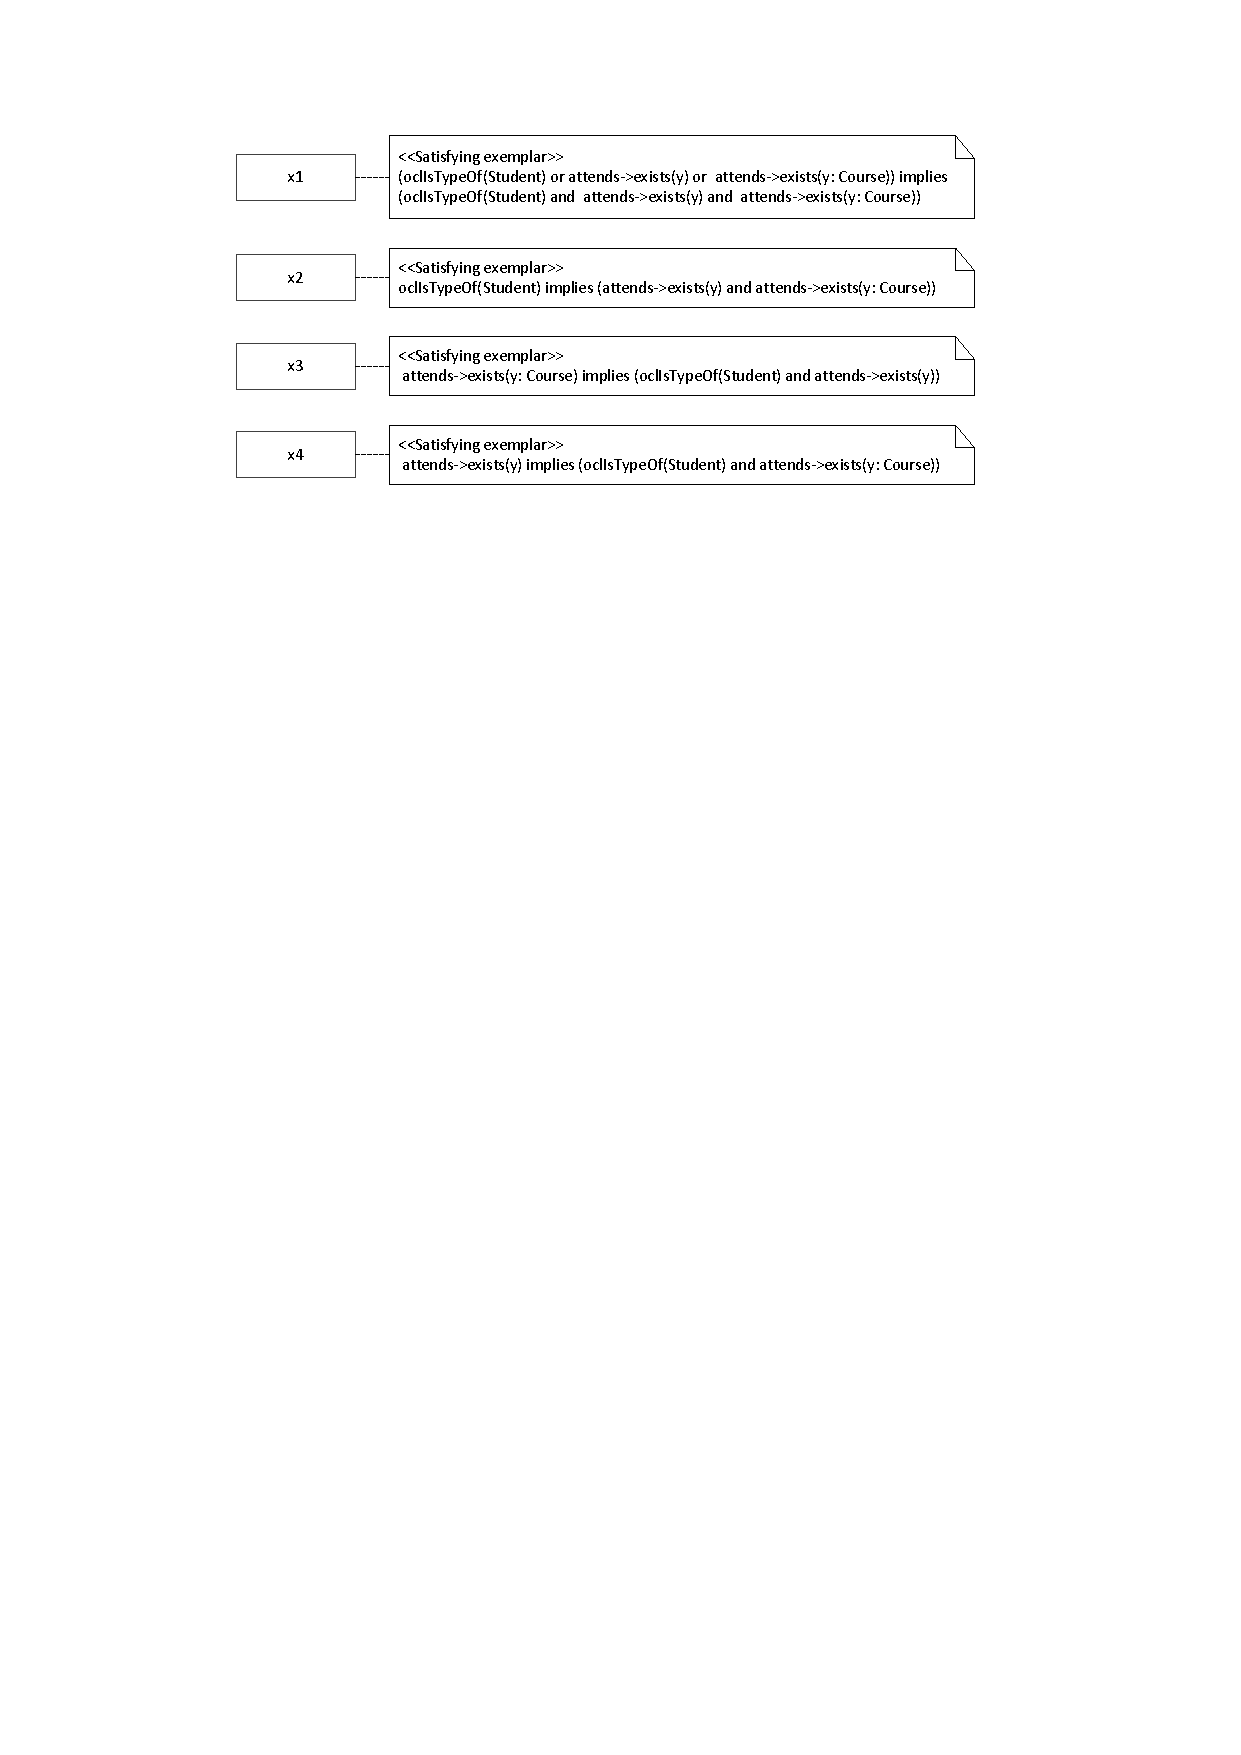
\includegraphics[trim = 30mm 215mm 30mm 15mm, clip, scale=0.9]{./ArmstrongOD_Student_AttendsSomeThing_AttendsSomeCourse.pdf}
 	\caption{Object diagram corresponding to Table~\ref{tab_ArmstrongOD_Student_AttendsSomeThing_AttendsSomeCourse}}
 		\label{fig_ArmstrongOD_Student_AttendsSomeThing_AttendsSomeCourse}
 \end{figure}  
 
 
  To analyse how the $\mathsf{Student}$ class relates to its $\mathsf{attends}$ attribute, we generate an Armstrong ABox for $\mathcal{T}_2^{UML}$ and $M = \{\mathsf{Student}, \exists \mathsf{attends}.\top\}$. This Armstrong ABox is given in Table~\ref{tab_ArmstrongOD_Student_AttendsSomeThing}. It confirms that in our application domain an individual that attends something is a student (as indicated by the satisfying exemplar defined by $x_3$), and that a student is an individual that attends something (see $x_2$). Even though this Armstrong ABox describes our application domain accurately, we may want to ensure that a student attends courses and that someone that attends courses is a student.
  Recall that due to the $M$-permissible restriction, we cannot confirm that a student can only attend courses, nor that someone that only attends courses is a student (see Section~\ref{subsec_MPermissibleRestriction}). 
  
  We can confirm that someone that attends courses is a student, and that a student is someone that attends courses, by generating an Armstrong ABox for $\mathcal{T}_2^{UML}$ and $M = \{\mathsf{Student}, \exists \mathsf{attends}.\top,$ $\exists \mathsf{attends}.\mathsf{Course}\}$. The Armstrong ABox is given in Table~\ref{tab_ArmstrongOD_Student_AttendsSomeThing_AttendsSomeCourse} and the associated Armstrong object diagram is given in Figure~\ref{fig_ArmstrongOD_Student_AttendsSomeThing_AttendsSomeCourse}.  Figure~\ref{fig_ArmstrongOD_Student_AttendsSomeThing_AttendsSomeCourse} uses some OCL notation we have not encountered this far. $\mathsf{attends}\texttt{->}\mathsf{exists(y)}$ states that for the instance $x_1$ the set represented by $\mathsf{attends}$ must contain at least one instance. No explicit type information is stipulated for $y$. $\mathsf{attends}\texttt{->}\mathsf{exists(y: Course)}$ states that for instance $x_1$ the $\mathsf{attends}$ set must contain at least one instance of type $\mathsf{Course}$.  
  The satisfying exemplar defined by individual $x_3$ confirms that an individual that attends a course necessarily is a student that attends something, while the satisfying exemplar defined by individual $x_2$ confirms that students necessarily attend courses.

  
 \subsection{Limitations of Armstrong ABoxes for $\mathcal{ALC}$ TBoxes for UML Class Diagrams}
 In Section~\ref{subsec_ArmstrongABoxLimitations} we have already discussed the limitations of Armstrong ABoxes. Here we want to briefly relate these limitations to the validation of UML class diagrams using Armstrong ABoxes. For this purpose we will refer to Figure~\ref{fig_UniversityClassDiagramIdeal}, which is an accurate description of our application. We highlight some key features of this diagram:
\begin{itemize}
	\item The $1..1$ multiplicity enforces that a course must be taught by exactly one teacher.
	\item The $\mathsf{UGStudent::attends}$ association is a subset of the $\mathsf{Student::attends}$ association, which enforces that undergraduate students can only attend undergraduate courses.
	\item The $\mathsf{PGStudent::attends}$ association is a subset of the $\mathsf{Student::attends}$ association for which the OCL constraint enforces that postgraduate students must attend at least one postgraduate course. 
\end{itemize}

    \begin{figure}
	%trim option's parameter order: left bottom right top
	\centering 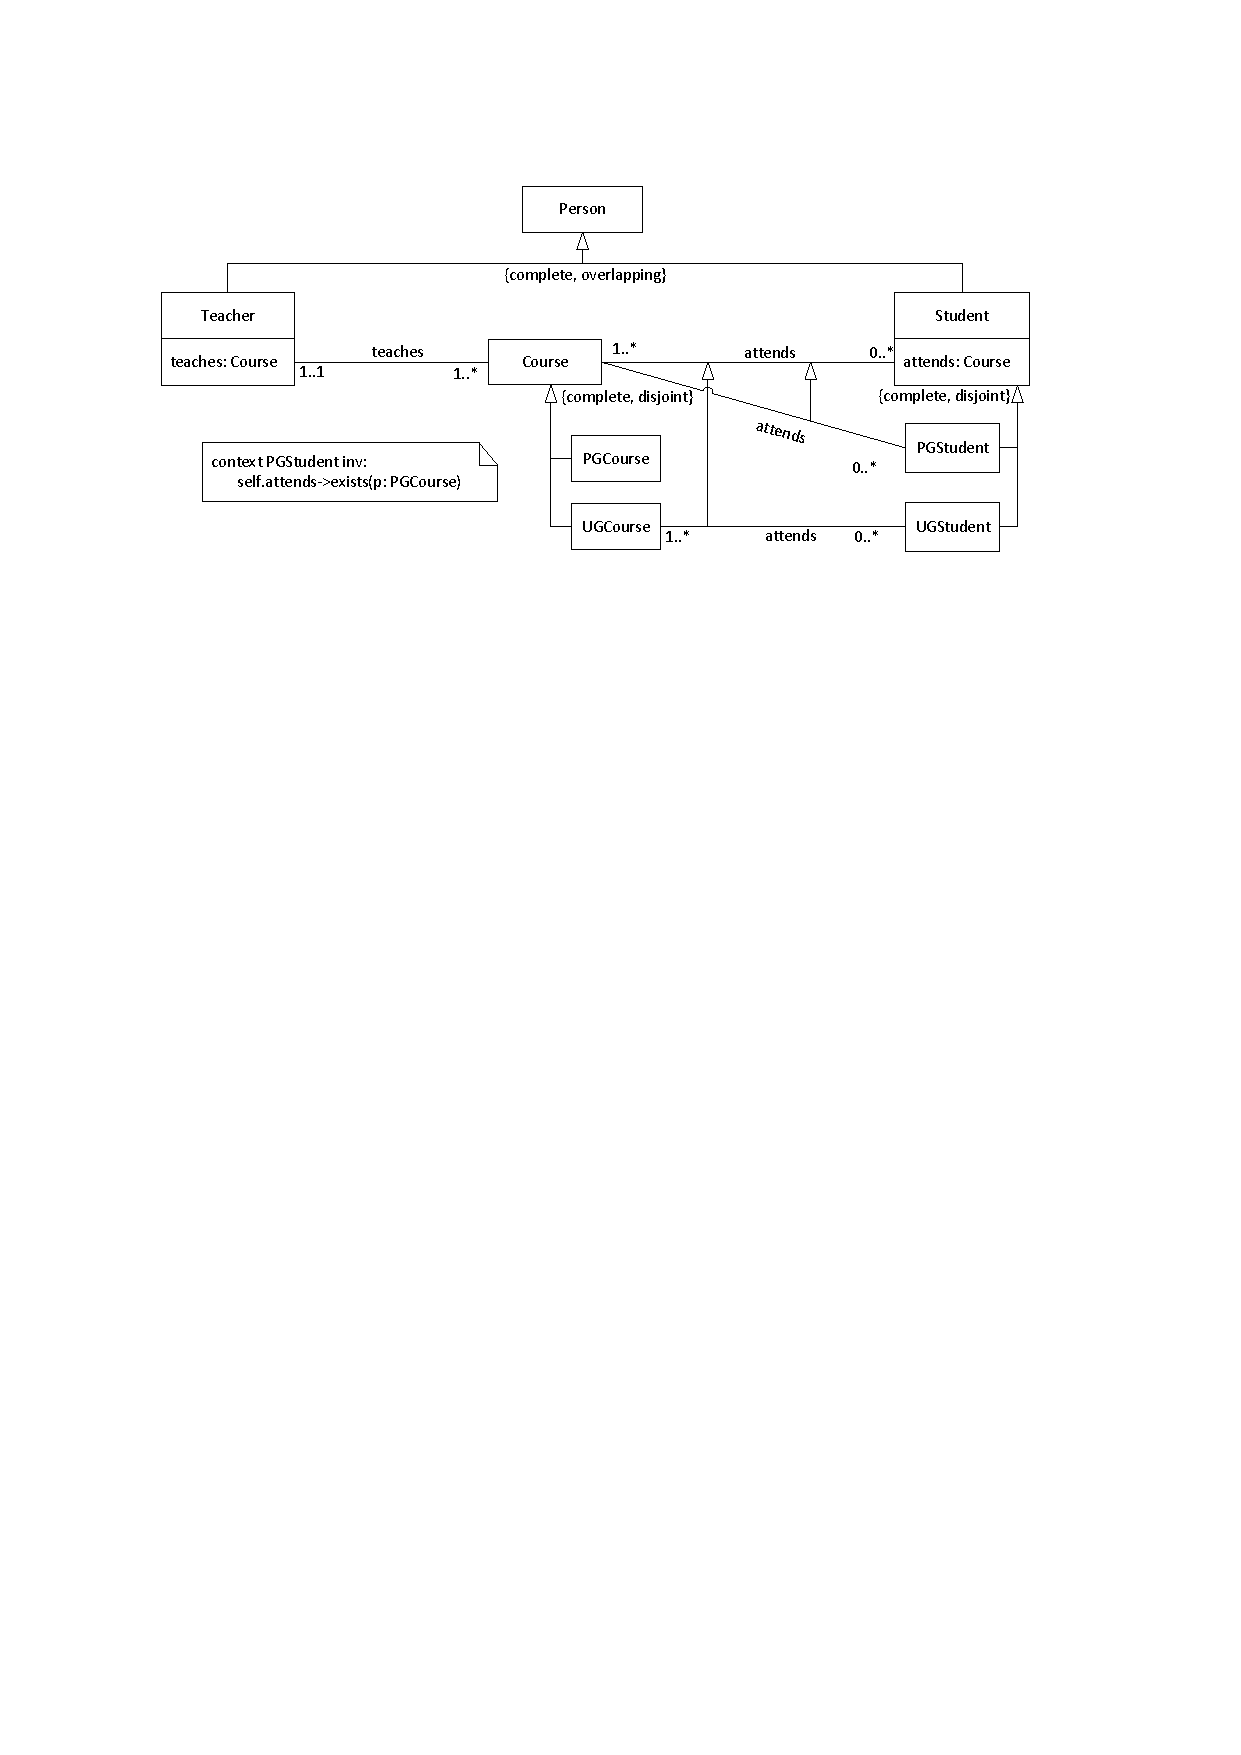
\includegraphics[trim = 25mm 200mm 30mm 15mm, clip, scale=0.9]{./UniversityClassDiagramIdeal.pdf}
	\caption{A UML class diagram that describes the application domain accurately}
	\label{fig_UniversityClassDiagramIdeal}
	\end{figure}
 
 We now discuss UML class diagram features for which the Armstrong ABox for $\mathcal{ALC}$ TBoxes formalization cannot cater.
  \begin{description}
  	\item[Associations in both direcions] In Figure~\ref{fig_UniversityClassDiagramIdeal} we can validate that teachers must teach at least one course. However, since $\mathcal{ALC}$ does not support inverse roles, we cannot ensure that a course is taught by at least one teacher. 
 	\item[Arbitrary multiplicities] In Section~\ref{subsec_ArmstrongABoxesAppliedToUML} we have given examples of how Armstrong ABoxes can be used to validate multiplicities like $1..*$, as in the case of teachers teaching at least one course. However, we cannot validate arbitrary multiplicities like for example $2..5$ or $1..1$. To validate a multiplicity like $2..5$ the Armstrong ABox formalization has to be extended to include qualified number restrictions. To support a multiplicity like $1..1$ the Armstrong ABox formalization must be extended with functional role restrictions, or qualified number restriction of which functional role restrictions is a subset.
 	\item[Association inheritance] Since $\mathcal{ALC}$ does not support role hierarchies, we cannot deal with association inheritance as seen in Figure~\ref{fig_UniversityClassDiagramIdeal} between $\mathsf{PGStudent::attends}$ and $\mathsf{Student::attends}$, as well as between $\mathsf{PGStudent::attends}$ and $\mathsf{Student::attends}$.
 	\item[Attibute types/Association ends] In Figure~\ref{fig_UniversityClassDiagramIdeal} the semantics of attribute types (association ends) enforces for example that students must attend courses and undergraduate students must attend undergraduate courses. Due to the $M$-permissible restriction, we cannot use Armstrong ABoxes to validate these as explained in Section~\ref{subsec_MPermissibleRestriction}. Extending the Armstrong ABox formalization to support inverse roles is one possible way around this limitation.
 \end{description} 

 \subsection{Applying Armstrong ABoxes for $n$-ary Relations to UML Class Diagrams}
    
   
   
        
 
  \bibliographystyle{amsplain}
  \bibliography{./BibliographicDetails_v.0.1}
 
\end{document}
